
\def\fmsnesl{SNESL\textsubscript{0}}
\def\fmsvcode{SVCODE\textsubscript{0}}



% \def\seval#1#2#3#4{\left\langle#1,#2 \right\rangle \Da^{#3} #4} 
% add cost
\def\seval#1#2#3#4#5{\left\langle#1,#2 \right\rangle \Da^{#3} #4 \ \$ \ #5} 
\def\sevalf#1#2#3#4{{\lcall}(#1,...,#2) \Da^{#3} #4}
\def\sevalfg#1#2#3#4{#1(#2) \Da^{#3} #4}

% Evaluation
%\def\Eval#1#2#3{#1 \Env #2 \Eva #3 }  % without cost
\def\Eval#1#2#3#4{#1 \Env #2 \Eva #3 \ \$ \ #4 } 


%typing
\def\Type#1#2#3{#1 \Env #2 : #3 } 
\def\Typef#1#2#3{#1 : (#2) \rightarrow #3}
\def\TypeV#1#2{#1 : #2}

%value representation
\def\ValRep#1#2#3{ #1 \triangleright_{#2} #3}

%value transback

\def\Vtransb#1#2#3#4{#1 \triangleleft_{#2} #3,#4}

\def\wf#1{\Vdash #1} %well-formed


\def\etail#1#2{\< #1 | \ #2 \ \'>}  % element and a tail vector

\def\PRName#1{\textsc{I-#1}}
\def\MI{\mathcal{I}}  % prefix rule


\chapter{Formalization}


%TODO add cost perservation
In this chapter, we will present the formal proof of the correctness of the translation for the language \fmsnesl \ , a core subset of \mysnesl.
First its formal definition and semantics will be given.
Then \fmsvcode, the target language of \fmsnesl \ , is defined, and proofs of some of its properties including freshness and determinism are given.
Note that as the first step to prove the full language, we only consider the eager semantics of this target language here.
The value representation and translation from \fmsnesl \  \ to \fmsvcode \ are also formalized.
Finally, we put emphasis on the proof of the main correctness theorem of this language.



\section{\fmsnesl}

The language \fmsnesl \  \ we will prove in this chapter is a subset of \mysnesl \ with its core semantics. 
The simplifications we have made from \mysnesl \  to \fmsnesl \  \ is listed below:
\begin{itemize}
	\item only one primitive type $\int$ 
	\item no pair types or zip-like comprehensions
	\item selected built-in functions 
	\item no restricted comprehension
	\item no user-defined functions
\end{itemize}


\subsection{Syntax}

\noindent (1) The types of \fmsnesl \  \ are: 
$$\tau ::= \int \ | \ \tseq{\tau_1}$$

\noindent (2) The synatx of \fmsnesl \  \ values : 
$$ n \in \mathbb{Z} $$
$$ v::= n \ | \ \{\replc{l}{v}\}$$

\noindent (3) The syntax of \fmsnesl \  \  \ expressions and the built-in functions are shown in Figure~\ref{fig:fmsnesl-exps}. 


\fig{
\begin{alignat*}{2}
& e &&::=  x  \tag{variable} \\
&   && \quad | \ \Let{x}{e_1}{e_2} \tag{let-binding}\\
&   && \quad | \ \hcall{\Tupk{x}}  \tag{built-in function call} \\
&   && \quad | \ \Comp{e}{x}{y}{\usevarsk} \tag{general comprehension} \\
\\
& \hcall && ::= \*{const}_n \ | \ \*{iota} \ | \ \*{plus} 
\end{alignat*}
}{\fmsnesl \  \  expressions and built-in functions \label{fig:fmsnesl-exps}}


Note that constants now are generated by calling the built-in function $\constn{n}()$ to limit the number of expression forms.
Also, the arguments of built-in functions as well as the input sequence in general comprehension are variables instead of expressions; we can simply convert the general forms of these expressions into the restricted forms by adding let-bindings for the variables. 
For example, the expression $\Comp{x+y}{x}{\&5}{y}$ in a general form can be turned to
\begin{alignat*}{2}
\*{let} & \ x_1 = \const{5} \ \*{in} \\
& \*{let} \ x_2 =  \iota{x_1} \ \*{in} \\
& \qquad \{ \plus{x}{y} :  x \ \*{in} \ x_2 \ \*{using}  \ y \}
\end{alignat*} 




\subsection{Typing rules}
\begin{itemize}
	
	\item Expression typing rules:\\
	
	\Jug{\Type{\Gam}{e}{\tau}}
	
	\PT{
		\AxiomC{}
		\RiLa{(\Gam(x) = \tau)}
		\UC{\Type{\Gam}{x}{\tau}}
	}
	\PT{
		\AC{\Type{\Gam}{e_1}{\tau_1}}
		\AC{\Type{\Gam[x \|-> \tau_1]}{e_2}{\tau}}
		\BC{\Type{\Gam}{\Let{x}{e_1}{e_2}}{\tau}}
	}\\[2ex]
	
	
	\PT{
		\AC{\Typef {\hcall} {\replc{k}{\tau}} {\tau}}
		\RiLa{((\Gam(x_i)= \tau_i)^k_{i=1})}
		\UC{\Type{\Gam}{\hcall{\Tupk{x}}}{\tau}}
	}\\[2ex]
	
	\PT{
		\AC{\Type{[x \|-> {\tau_1}, \k{x_i \|-> \int}]}{e}{\tau}}
		\RiLa{(\Gam(y)=\tseq{\tau_1}, \k{\Gam(x_i) = \int})}
		\UC{\Type{\Gam}{\Comp{e}{x}{y}{\usevarsk}}{\tseq{\tau}}}
	}\\[2ex]
	
	
\item  Built-in functions typing rules:\\

   \Jug{\Typef {\hcall} {\replc{k}{\tau}} {\tau}}
	
	\PT{\Axiom{\Typef{\constn{n}}{}{\int}}}
	\PT{\Axiom{\Typef{\iotan}{\int} {\tseq{\int}}}}
	\PT{\Axiom{\Typef{\plusn}{\int,\int} {\int}}}
	
	% value types
	\item Value typing rules: \\
	
	\Jug{\TypeV{v}{\tau}}
	
	\PT{\Axiom{\TypeV{n}{\int}}}
	\PT{
		\AC{(\TypeV{v_i}{\tau})^l_{i=1}}
		\UC{\TypeV{\{\replc{l}{v}\}}{\tseq{\tau}}}
	}
	
\end{itemize}


\subsection{Semantics}

%TODO explain |v| and cost 

\begin{itemize}
\item Expression evaluation rules:
	
	\Jug{\Eval{\rho}{e}{v}{W}}
	\PT{
		\AxiomC{}
		\RiLa{(\rho(x)=v)}
		\UC{\Eval{\rho}{x}{v}{0}}
	}
	\PT{
		\AC{\Eval{\rho}{e_1}{v_1}{W_1}}
		\AC{\Eval{\rho[x \|-> v_1]}{e_2}{v}{W_2}}
		\BC{\Eval{\rho}{\Let{e_1}{x}{e_2}}{v}{W_1+ W_2}}	
	}\\[2ex]	
	\PT{
		\AC{\EvalF\hcall{\replc{k}{v}}{v}}
		\RiLa{((\rho(x_i)=v_i)^k_{i=1})}
		\UC{\Eval{\rho}{\hcall{\Tupk{x}}}{v}{(\sum_{i=1}^{k}|v_i|) + |v|} }
	}\\[2ex]
	
	\PT{
		\AC{(\Eval{[x \|-> {v_i}, x_1 \|-> n_1,...,x_k \|-> n_k]}{e}{v_i'} {W_i})^l_{i=1}}
		\RiLa{\left(
			\begin{aligned}
				& \rho(y)=\{\replc{l}{v}\} \\
				& \k{\rho(x_i) = n_i}
			\end{aligned}
			\right)}
		\UC{\Eval{\rho}{\Comp{e}{x}{y}{\usevarsk}}
			     {\{\replc{l}{v'}\}}      
			     {1 + l\cdot k + \sum_{i=1}^{l}W_i}}
	}\\[2ex]
	
\item Built-in function evaluation rules:

  \Jug{\EvalF\hcall{\replc{k}{v}}{v}}
	
	\PT{\Axiom{\EvalF{\constn{n}}{}{n}}}
	\PT{\AC{}
		\RiLa{(n \ge 0)}
		\UC{\EvalF{\iotan}{n}{\{0,1,...,n-1\}}}} \\[2ex]
	
	\PT{\AC{} 
		\RiLa{(n_3= n_1+n_2)} 
		\UC{\EvalF{\plusn}{n_1,n_2}{n_3}}}
	
\end{itemize}


\section{\fmsvcode}
The target language of \fmsnesl \  is also a subset of SVCODE presented in the last chapter. 
We will call it  \fmsvcode.

\subsection{Syntax}
In this minimal language, a primitive stream $\a$ can be a vector of booleans, integers or units, as the following grammar shows:

$$b \in \mathbb{B} = \{\T,\F \}$$
$$ a ::= n \ | \ b \ | \ \unit$$
$$\b = \vrange{b_1}{b_i}$$ 
$$\c = \vrange{()}{()} $$
$$\a = \vrange{a_1}{a_i}  $$ 

\hspace{1cm}

The syntax of \fmsvcode \  is given in Figure~\ref{fig-svcode-grammar}.


\begin{figure}[H] \large
	\begin{alignat*}{2}
	&p  && :: = \ \epsilon \\ 
	&   &&\ \ | \ \sdef{\s}{\psi(s_1,...,s_k)} \\
	&   &&\ \ | \ \withctrl{\s}{p_1}{\Sin}{\Sout} \\
	&   &&\ \ | \ p_1;p_2  \\
	\\
	&\s && ::= 0 \ | \ 1 \ ... \in \SId  = \mathbb{N}   \tag{stream ids}\\
	\\
	& \psi \ && ::= \consta{a} \ | \ \toflag  
	\ | \ \usum \ | \ \maptwo{\oplus} \ | \ \scan_{n_0} \ | \ \distr  \tag{Xducers} \\
	& \oplus \ && :: = + \ | \ - \ | \ \times \ | \ \div \ | \ \% \ | \ ...  \tag{binary integer operations}\\
	\\
	&  \S && ::= \{\s_1,..., \s_i\} \in \sset  \tag{a set of stream ids}
	\end{alignat*}
	\caption{Abstract syntax of \fmsvcode \  \label{fig-svcode-grammar}}
%TODO fix Xducer maptwo?
\end{figure}


The function $\texttt{dv}$ returns the set of defined variables of a given \fmsvcode \  program.

\begin{alignat*}{2}
&\dv{\epsilon} && =  \emptyset \\
&\dv{\sdef{\s}{\psi(s_1,...,s_k)}} && =  \{s\} \\
&\dv{\withctrl{\s_c}{p_1}{\Sin}{\Sout}} && =   \Sout \\
&\dv{p_1;p_2} && =  \dv{p_1} \cup \dv{p_2} \\
\end{alignat*}

Correspondingly, $\texttt{fv}$ returns the free variables set.

\begin{alignat*}{2}
&\FV{\epsilon} && = \emptyset \\
&\FV{\sdef{\s}{\psi(s_1,...,s_i)}} && = \{s_1,...,s_k\}\\
&\FV{\withctrl{\s_c}{p_1}{\Sin}{\Sout}} && = \{s_c\} \cup \Sin \\
&\FV{p_1;p_2} && = \FV{p_1} \cup (\FV{p_2} - \dv{p_1}) \\
\end{alignat*}


\begin{defi}[\textbf{Well-formedness}]
	p is a well-formed SVCODE program, written as $\Vdash p$, if it can be shown by the following rules:
\end{defi}
  \Jug{\wf{p}}
	
	\PT{\Axiom{\wf{\epsilon}}}
    \PT{ \RiLa{(s\notin \{s_1,...,s_k\})}
   		\Axiom{\wf{\sdef{s}{\lcall(s_1,...,s_k)}}}}\\[3ex]
   	
   	\PT{\AC{\wf{p_1}}
    	\RiLa{\left(
    		\begin{aligned}
    			&\FV{p_1} \subseteq \Sin \\
    			&\Sout \subseteq \dv{p_1} \\
    			&(\{\s\} \cup \Sin)  \cap \Sout = \emptyset
    		\end{aligned}
    		 \right)} 
    	\UC{\wf{\withctrl{s}{p_1}{\Sin}{\Sout}}}  
   	}\\[3ex]
   
   \PT{\AC{\wf{p_1}}
   	   \AC{\wf{p_2}}
   	   \RiLa{\left(
   	   	\begin{aligned}
   	   		(\FV{p_1} \cup \dv{p_1}) \cap \dv{p_2} = \emptyset \\
   	   	\end{aligned}
      	\right)}  	  
       \BC{\wf{(p_1;p_2)}}
   }\\[3ex]
   

An immediate property of this language is that the defined variables of a \emph{well-formed} \fmsvcode \  program are always fresh. In other words, there is no overlapping between the free variables and the newly generated ones.


\begin{lem}[\textbf{Freshness}]
	If $p$ is well-formed, then  $\FV{p} \cap \dv{p} = \emptyset $. 
\end{lem}

The proof is straightward by induction on the derivation of $\wf{p}$.

%TODO well-formed 

\subsection{Instruction semantics}

Before showing the semantics, we first introduce some notations and operations about streams for convenience.
\begin{nota}
	Let $\< a_0 | \a \'>$ denote a non-empty stream $\< a_0,a_1,...,a_l \'>$ for some $\a = \< a_1,...,a_l \'>$. 
\end{nota}


\begin{nota}[\textbf{Stream concatenation}]
	$\vapp{\vrange{a_1}{a_i}} {\vrange{a_1'}{a_j'}} = \langle a_1,...,a_i,a_1',...,a_j' \rangle $ \\
\end{nota}

\begin{nota}[\textbf{Stream length}]
	For a stream $\a = \< a_1,...,a_l \'>$, $|\a|$ = l. \\
\end{nota}

The operational semantics of \fmsvcode \  is given in Figure~\ref{fig-svcode-semantics}.
The runtime environment or store $\sgm$ is a mapping from stream variables to vectors:
$$\sgm = [\s_1 \|-> {\a_1},...,\s_i \|-> {\a_i}]$$
The control stream $\c$, which is a vector of units, indicates the parallel degree of the computation, as we have discussed in the last chapter. 
It is worth noting that only in the rule $\PName{Wc-Nonemp}$ the control stream gets changed.


\begin{figure}[H]\large 
	
	\Jug{\seval{p}{\sgm}{\c}{\sgm'}{W}}\\
	
	
	\PT{\LeLa{\PName{Empty:}}			   
		\Axiom{\seval{\epsilon}{\sgm}{\c}{\sgm}{0}}
	} \\[2ex]
	
	\PRule{Xducer}{\PT{\AC{\sevalf{\a_1}{\a_k}{\c}{\a}}
			\RiLa{((\sgm(\s_i) = \a_i)^k_{i=1})}
			\UC{\seval{\sdef{\s}{\lcall\Tupk\s}}{\sgm}{\c}{\sgm[\s \|-> \a]}{(\sum_{i=1}^{k}|\a_i|) + |\a|}}
	}} \\[4ex]
	
	\PT{ \LeLa{\PName{Wc-Emp:}}
		\AC{}
		\RiLa{
			\left(
			\begin{aligned}
				&\forall s \in \{s_c\} \cup \Sin. \sgm(s) = \emptyv \\
				&\Sout = \{s_1,...,s_k\}
			\end{aligned}
			\right)}
		\UC{\seval{\withctrl{\s_c}{p_1}{\Sin}{\Sout}}{\sgm}{\c}{\sgm[\k{\s_i \|-> \emptyv}]}{1}}
	}\\[2ex]
	$\PName{Wc-Nonemp}:$\\
		\PT{
			\AC{\seval{p_1}{\sgm}{\c_1}{\sgm''}{W_1}}
			\RiLa{\left(
				\begin{aligned} 
					&\sgm(\s_c)= \c_1 \ne \emptyv \\
					&\Sout = \{s_1,...,s_k\}
				\end{aligned}\right)}
			\UC{\seval{\withctrl{\s_c}{p_1}{\Sin}{\Sout}}{\sgm}{\c}{\sgm[\k{\s_i \|-> \sgm''(\s_i)}]} {W_1+1} }
	}\\[4ex]
	
	\PRule{Seq}{\PT{
			\AC{\seval{p_1}{\sgm}{\c}{\sgm''} {W_1} }
			\AC{\seval{p_2}{\sgm''}{\c}{\sgm'} {W_2} } 	
			\BC{\seval{p_1;p_2}{\sgm}{\c}{\sgm'} {W_1 + W_2} }
	}}
	
	\caption{\fmsvcode \  semantics}
	\label{fig-svcode-semantics}
\end{figure}

The rule $\PName{Empty}$ is trivial, an empty program doing nothing on the store. 

The rule $\PName{Xducer}$ adds the store a new stream binding where the bound vector is generated by a specific Xducer. The detailed semantics of Xducers will be given in the next subsection. 

The rules $\PName{Wc-Emp}$ and $\PName{Wc-Nonemp}$ together show two possibilities for interpreting a \wc instruction:
\begin{itemize}
	\item if the new control stream $\s_c$ and the streams in $\Sin$, which includes the free variables of $p_1$, are all empty, then just bind empty vectors to the stream ids in $\Sout$, which is a part of the defined streams of $p_1$.
	\item otherwise execute the code of $p_1$ as usual under the new control stream, ending in the store $\sgm''$; then copy the bindings of $\Sout$ from $\sgm''$ to the initial store. 
\end{itemize}

\subsection{Xducer semantics}
The semantics of Xducers are abstracted into two levels: the $general$ level and the $block$ level. The general level summarizes the comman property that all Xducers share, and the block level describes the specific behavior of each Xducer. 

Figure~\ref{fig-xducer-semantics} shows the semantics at the general level. 


\begin{figure}\large
	
	\Jug{\sevalf{\a_1}{\a_k}{\c}{\a}} \\
		
	\PRule{X-Loop}{\PT{
			\AC{\block{\a_{11}}{\a_{k1}}{\a_{01}}}
			\AC{\sevalf{\a_{12}}{\a_{k2}}{\c_0}{\a_{02}}}
			\RiLa{((\vapp{\a_{i1}}{\a_{i2} = \a_i})^k_{i=0})}
			\BC{\sevalf{\a_1}{\a_k}{\< () | \c_0 \rangle}{\a_0}}
	}}\\[4ex]
	
	\LeLa{\PName{X-Termi:}} 
	\Axiom{\sevalf {\emptyv_1} {\emptyv_k} \emptyv \emptyv}
	\DisplayProof \footnotemark	
	\caption{General semantics of \fmsvcode \  Xducers \label{fig-xducer-semantics}}
\end{figure}
\footnotetext{For notational convenience, in this thesis we add subscripts to a sequence of constants, such as $\emptyv, \F, 1$, to denote the total number of these constants.}

There are only two rules for the general semantics. 
They together say that the output stream of a Xducer is computed in a ``loop" fashion, where the 
iteration uses specific block semantics of the Xducer and the number of iteration is the unary number that the control stream represents, i.e., the length of the control stream. 
In the parallel setting, we prefer to call this iteration a $block$. 
Recall the control stream is a representation of the parallel degree of the computation, then a block consumes exact one degree. 
It is worth noting that all these blocks are data-independent, which means they can be executed in parallel. 
So the control stream indeed carries the theoretical
maximum number of processors we need to execute the computation most efficiently, if the computation within the block cannot be parallelized further. \\


After abstracting the general semantics, the remaining work of formalizing the specific semantics of Xducers within a block becomes relatively clear and simple. The block semantics are defined in Figure~\ref{fig:xducer-bl-seman}. 

\begin{figure}[H]\large
	\def\'>{\rangle}
	
	\Jug{\block{\a_1}{\a_k}{\a}} \\
	
	\PT{\LeLa{\PName{X-Const:}} 
		\Axiom{\blockf{\consta{a}}{}{\singl{a}}}
	}
	\PT{\LeLa{\PName{X-ToFlags:}} 
		\Axiom{\blockf{\toflag}{\singl{n}}{\< \F_1,...,\F_n,\T \'>}} } \\[3ex]
	\PRule{X-MapTwo}{\PT{\AC{}
			\RiLa{(n_3= n_1 \oplus n_2)}
			\UC{\blockf{\maptwo{\oplus}}{\singl{n_1}, \singl{n_2}} {\singl{n_3}}}
	}} \\[3ex]
	
	%--- UsumF
	\PRule{X-UsumF}{
		\PT{\AC{\blockf{\usum}{\b}{\a}}
			\UC{\blockf{\usum}{ \<\F|\b \'>}{\<()|\a\'>}}
		}
	}
	\PT{\LeLa{\PName{X-UsumT:}} \Axiom{\blockf{\usum}{\oT}{\emptyv}}}
	\\[3ex]

	\PRule{X-ScanF}{
		\PT{\AC{\blockf{\scan_{n_0+n}}{\b,\a}{\a'}}
			\UC{\blockf{\scan_{n_0}}{\<\F|\b \'>, \<n|\a\'>}{\<n_0|\a'\'>}}
		}		
	}\\[3ex]

	\PT{\LeLa{\PName{ScanT:}} 
		\Axiom{\blockf{\scan_{n_0}}{\oT, \emptyv}{\emptyv}}
	}\\[3ex]
		
	\PRule{X-DistrF}{
		\PT{\AC{\blockf{\distr}{\b, \<n\'>}{\a}}
			\UC{\blockf{\distr}{\<\F|\b \'>, \<n\'>}{\<n|\a \'>}}
		}
	}
	\PT{\LeLa{\PName{X-DistrT:}}\Axiom{\blockf{\distr}{\oT,\<n\'>}{\emptyv}}}\\[1ex]
		
\caption{Block semantics of  Xducers \label{fig:xducer-bl-seman}}
\end{figure}



%\begin{itemize}
%	\renewcommand{\labelitemi}{$-$}
%	\item $\constaf{a}$ outputs the const $a$ until the control stream reaches EOS.
%	
%	\begin{example} \emph{$\constaf{3}$ with control stream $\c = \<(),()\'>$:}\\
%		\begin{center}
%			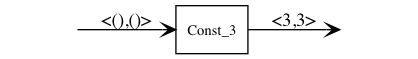
\includegraphics[width=0.6\textwidth]{fig/const3.png}
%		\end{center}
%	\end{example}
%	
%	\item $\toflagf{\singl{n}}$ first outputs $n$ $\F$s, then one $\T$.
%	
%	\begin{example} \emph{$\toflagf{\<2,0\'>}$:}\\
%		\begin{center}
%			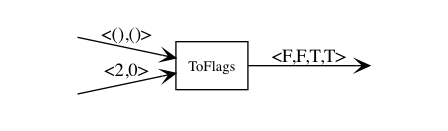
\includegraphics[width=0.6\textwidth]{fig/toflag.png}
%		\end{center}
%	\end{example}
%	
%	\item $\maptwof{\oplus}{\singl{n_1}}{\singl{n_2}}$ outputs 
%	the binary operating result of $\oplus$ on $n_1$ with $n_2$. 
%	
%	\begin{example} \emph{$\maptwof{+}{\<3,2\'>}{\<1,1\'>}$:}\\
%		\begin{center}
%			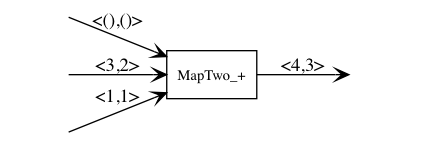
\includegraphics[width=0.6\textwidth]{fig/maptwo.png}
%		\end{center}
%	\end{example}
%	
%	
%	
%
%\end{itemize}
%



As mentioned before, we can consider a block  as the minimum computing unit assigned to a single processor. This is reasonable for
Xducers such as $\consta{a}$ and $\maptwo{\oplus}$, because
they are already sequential at the block level. 

However, some other Xducers, such as $\usum$, can be parallelized further inside a block.
As we have implemented more Xducers than shown here, we find that computations on unary numbers within blocks are common, which is mainly due to the value representation strategy we use, but also more difficult to be regularized.
For the scope of this thesis, the block semantics we have shown are already relatively clear and simple enough to reason about, and the unary level parallelism can be investigated in future work. 



%Or if we want to use $unary$ semantics maybe for later: \\
%\begin{mdframed}
%\PT{
%	\AC{\unary{\singl \F}{\a_{k1}}{\a_1}}
%	\AC{\block{\a_{12}}{\a_{k2}}{\a_2}}
%	\RiLa{(\a = \vapp{\a_1}{\a_2})}
%	\BC{\block{\vapp {\singl\F} {\a_{12}}} {\vapp {\a_{k1}} {\a_{k2}}}{\a}}
%}\\[2ex]
%
%\PT{
%	\AC{\unary{\oT} {\a_k}{\a}}
%	\UC{\block{\oT}{\a_k} \a}
%}\\[2ex]
%
%\begin{itemize}
%\item Transducer $unary$ semantics:\\ 
%
%\Jug{\unary{\singl b}{\a_k}{\a}}
%
%\PT{ \Axiom{\usum(\oF) \dda \vunit}}
%\PT{\Axiom{\usum(\oT) \dda \emptyv }} \\[1ex]
%
%
%%loopuv
%\item Transducer block with $accumulator$: \\
%
%\Jug{\blockv{n}{\a_1}{\a_k}{\a}}
%\PT{
%	\AC{\unaryv{n_0} {\singl \F}{\a_{k1}}{n_0'} {\singl{n_1}}  }
%	\AC{\blockv{n_0'}{\a_{12}}{\a_{k2}}{\a_2}}
%	\BC{\blockv{n_0} {\vapp {\singl\F} {\a_{12}}} {\vapp {\a_{k1}} {\a_{k2}}}{\vapp {\singl{n_1}} {\a_2}} }
%}\\[2ex]
%
%\PT{
%	\AC{\unaryv {n_0} \oT {\a_k} {} {\a}}
%	\UC{\blockv {n_0} \oT {\a_k} {\a} }
%}
%
%\item Transducer unary with $accumulator$: \\
%
%\Jug{\unaryv{n}{\oF}{\a_k}{n'}{\a}}
%
%\PT{\Axiom{\scan_{n_0}(\oF,{\singl{n}}) \dda^{n_0+n} {\singl{n_0}} }} \\
%
%\Jug{\unaryv{n}{\oT}{\a_k}{}{\a}}
%
%\PT{\Axiom{\scan_{n_0}(\oT, \emptyv) \dda {\emptyv} }}
%\end{itemize}
%\end{mdframed}

\subsection{\fmsvcode \ determinism}

We now present  how we prove a well-formed \fmsvcode \  program is deterministic.\\

\begin{defi}[\textbf{Stream prefix}]
	$\a$ is a $prefix$ of $\a'$, written $\a \prefix \a'$, if one of the following rules applys: \\
	
	\emph{\Jug{\a \prefix \a'}}
	\PT{\LeLa{\PRName{Emp:}} \Axiom{\emptyv \prefix \a' }}
	\PRName{Nonemp:}{
		\PT{
			\AC{\a \prefix \a'}
			\UC{\<a_0 \ | \ \a \'> \prefix \<a_0 \ | \ \a' \'>}
	}}\\
	
\end{defi}

\begin{lem}\label{lem-app2pre}
	If $\a_1 {\++} \a_2 = \a$, then $\a_1 \prefix \a$.
\end{lem}
\begin{proof}
	The proof is straightforward by induction on $\a_1$: case $\a_1 = \emptyv$ and case $ \a_1 = \< a_0 \ | \ \a_1' \'>$ for some $\a_1'$.
\end{proof}

The following lemma says that a Xducer always knows how many elements it should consume and produce when it reads one element from the control stream, i.e., in one block, and these numbers are fixed in any block for the same Xducer.


\begin{lem}[\textbf{Blocks are self-delimiting}] \label{lem-block-unique}
	If
	\begin{enumerate}[(i)]
		\item $(\a_i' \prefix  \a_i \ by \ some \ derivation \ \MI_{i})^k_{i=1}$ and $\block{\a_1'}{\a_k'}{\a'}$ by some $\MP$, 
		\item $(\a_i'' \prefix \a_i \ by \ some \ derivation \ \MI'_{i})^k_{i=1}$ and
		$\block{\a_1''}{\a_k''}{\a''}$ by some $\MP'$.
	\end{enumerate} 
	then \begin{enumerate}[(i)]
		\item $(\a_i' = \a_i'')^k_{i=1}$ 
		\item $\a' = \a''$.
	\end{enumerate}
\end{lem}

\begin{proof}
	The proof is by induction on $\MP$. We show three cases 
	$\PName{-X-ToFlags}$, $\PName{-X-ScanT}$ and $\PName{-X-ScanF}$ here; the others are analogous.
	\begin{itemize}
		\item Case $\MP$ uses $\PName{-X-ToFlags}$. \\
		Then
		$$	\PT{\LeLa{\MP =} 
			\Axiom{\blockf{\toflag}{\singl{n_1}}{\< \F_1,...,\F_{n_1},\T \'>}} }
		$$
		and 
		$$	\PT{\LeLa{\MP' =} 
			\Axiom{\blockf{\toflag}{\singl{n_2}}{\< \F_1,...,\F_{n_2},\T \'>}} }
		$$
		so $k=1, \a_1' = \singl{n_1}$, $\a' = \< \F_1,...,\F_{n_1},\T \'>$, and  
		$\a_1'' = \singl{n_2}$, $\a'' = \< \F_1,...,\F_{n_2},\T \'>$. \\
		Since both $\a_1'$ and $\a_1''$ are nonempty, $\MI_{1}$ and $\MI_{1}'$ must both use the rule $\PRName{Nonemp}$,
		which implies $n_1$ = $n_2$. 
		Then it is clear that $\a_1' = \a_1''$ and $\a' = \a''$, as required. 
		
		\item Case $\MP$ uses $\PName{-X-ScanT}$. \\
		Then 	
		$$\PT{\LeLa{\MP = } \Axiom{\blockf{\scan_{n_0}}{\oT, \emptyv}{\emptyv}}}$$
		so $k$=2, $\a_1' = \oT$. 
		Since $\a'_1$ is nonempty, then $\MI_{1}$ must use $\PRName{Nonemp}$, which implies the first element of $\a_1$ is $\T$. \\		
		There are two possibilities for $\MP'$:
		\begin{itemize}
			\item Subcase $\MP'$ uses $\PName{-X-ScanF}$.\\
			This subcase is impossible, because it requires $\a_1$ starts with a $\F$, which is contradictory to what we already know.
			
			\item Subcase $\MP'$ uses $\PName{-X-ScanT}.$ \\
			Then $$\PT{\LeLa{\MP' = } \Axiom{\blockf{\scan_{n_0}}{\oT, \emptyv}{\emptyv}}}$$
			So $\a''_1 = \oT = \a'_1$, $\a''_2 = \emptyv = \a'_2$, and $\a'' = \emptyv = \a''$, as required. 
			
		\end{itemize}
		
		
		\item Case $\MP$ uses $\PName{-X-ScanF}$. \\
		Then 
		$$\PT{\UCN{\MP_0}{\blockf{\scan_{n_0+n}}{\a'_{10},\a'_{20}}{\a_0'}}
			\LeLa{\MP = }
			\UC{\blockf{\scan_{n_0}}{\<\F|\a'_{10} \'>, \<n|\a'_{20}\'>}{\<n_0|\a'_0\'>}}
		}$$
	
		So $k$=2, $\a_1' = \<\F|\a'_{10} \'>$, and $\a_2' = \<n|\a'_{20}\'>$. 
		$\MI_{1}$ must use $\PRName{Nonemp}$, which implies the first element of $\a_1$ is $\F$. So $\a_1 = \< \F | \a_{10}\'>$ for some $\a_{10}$. 
		By the rule $\PRName{Nonemp}$, we have
			$$\PT{
				\AC{\a'_{10} \prefix \a_{10}}
				\UC{\<\F|\a'_{10} \'> \prefix \< \F | \a_{10}\'>}
			}$$
				
		Similarly, we can assume  $\a_2 = \<n |\a_{20} \'>$, and we must have $\a'_{20} \prefix \a_{20}$.
		Thus, \eq{eq-scan-determ-1}{
			( \a_{i0}' \prefix \a_{i0} )^2_{i=1}}
		There are two possibilities for $\MP'$:
		\begin{itemize}
			\item Subcase $\MP'$ uses $\PName{-X-ScanT}$.\\
			This subcase is impossible, because $\a_1$ does not start with a $\T$. 
			
			\item Subcase $\MP'$ uses $\PName{-X-ScanF}$.\\
			Then	
			$$\PT{\UCN{\MP_0'}{\blockf{\scan_{n_0+n}}{\a''_{10},\a''_{20}}{\a''_0}}
				\LeLa{\MP' = }
				\UC{\blockf{\scan_{n_0}}{\<\F|\a''_{10} \'>, \<n|\a''_{20}\'>}{\<n_0|\a''_0\'>}}
			}$$
			so $\a_1'' =  \<\F|\a''_{10} \'>, \a_2'' = \<n|\a''_{20}\'>$, $\a'' = \<n_0|\a''_0\'>$, 
			and it is easy to show  \eq{eq-scan-determ-2}{
				(\a''_{i0} \prefix \a_{i0} )^2_{i=1}}
			
			Here we first prove the following inner lemma: \\		
			if $(\a'_{i0} \prefix \a_{i0} )^2_{i=1}$ and $\blockf{\scan_{n_0}}{\a'_{10},\a'_{20}}{\a'}$ by some derivation $\MP_0$,
		    $(\a''_{i0} \prefix \a_{i0} )^2_{i=1}$ and $\blockf{\scan_{n_0}}{\a''_{10},\a''_{20}}{\a''}$,
			then $\a'_{10} = \a''_{10}, \a'_{20} = \a''_{20}$,  and $\a' = \a''$. \\
			The proof is by induction on $\MP_0$.  There are two subcases:
			for the case $\MP_0$ uses $\PName{-X-ScanT}$, the proof is analogous to the outer proof case $\MP$ uses  $\PName{-X-ScanT}$; for the case $\MP_0$ uses $\PName{-X-ScanF}$, the proof can be done by the inner IH. 	
			
			Then, by this inner lemma on $\eqref{eq-scan-determ-1}$ with $\MP_0$, 
			$\eqref{eq-scan-determ-2}$, $\MP_0'$, we get
			$(\a'_{i0} = \a''_{i0})^2_{i=1}$, and $\a'_0 = \a''_0$. \\
			Thus $\< \F |\a'_{10} \'> = \<\F | \a''_{10} \'>$, i.e., $\a'_1 = \a''_1$. 
			Likewise, $\a'_2 = \<n|\a'_{20}\'> = \<n|\a''_{20}\'> = \a''_2$, and  $\a' = \<n_0|\a'_0\'> = \<n_0|\a''_0\'> = \a''$, as required. 
			
		\end{itemize}
		
	\end{itemize}
\end{proof}


\begin{lem}[\textbf{Xducer determinism}] \label{lem-xducer-determ}
	If $\sevalfg{\lcall}{\replc{k}{\a}}{\c}{\a_0}$ by some derivation $\MP$,
	and $\sevalfg{\lcall}{\replc{k}{\a}}{\c}{\a'_0}$ by some derivation $\MP'$,
	then $\a_0 = \a'_0$.
\end{lem}

\begin{proof}
	The proof is by induction on the structure of $\c$. 
	\begin{itemize}
		\item Case $\c = \emptyv$ \\
		Then both $\MP$ and $\MP'$ must use $\PName{X-Termi}$:
		$$\PT{ 
			 \LeLa{\MP = \MP' = }
			 \Axiom{\sevalf {\emptyv_1} {\emptyv_k} \emptyv \emptyv}
			}$$
		so $\a_0 = \a_0' = \emptyv$, as required.
		
		\item Case $\c = \< () | \c_0 \'>$. \\		
		$\MP$ must use $\PName{X-Loop}$:
		$$\PT{
			\UCN{\MP_1}{\block{\a_{11}}{\a_{k1}}{\a_{01}}}
			\UCN{\MP_2}{\sevalf{\a_{12}}{\a_{k2}}{\c_0}{\a_{02}}}
			\LeLa{\MP = }
			\BC{\sevalf{\a_1}{\a_k}{\< () | \c_0 \rangle}{\a_0}}
		}$$
		where 
		\eq{eq-xdu-1}{(\vapp{\a_{i1}}{\a_{i2}} = \a_i)^k_{i=1}}
		\eq{eq-xdu-2}{\vapp{\a_{01}}{\a_{02}} = \a_0}
		Similarly,
		$$\PT{
			\UCN{\MP'_1}{\block{\a'_{11}}{\a'_{k1}}{\a'_{01}}}
			\UCN{\MP'_2}{\sevalf{\a'_{12}}{\a'_{k2}}{\c_0}{\a'_{02}}}
			\LeLa{\MP' = }
			\BC{\sevalf{\a_1}{\a_k}{\< () | \c_0 \rangle}{\a'_0}}
		}$$
		where
		\eq{eq-xdu-3}{(\vapp{\a'_{i1}}{\a'_{i2}} = \a_i)^k_{i=1}}
		\eq{eq-xdu-4}{\vapp{\a'_{01}}{\a'_{02}} = \a'_0}
		
		Using Lemma~\ref{lem-app2pre} on each of the $k$ equations of \eqref{eq-xdu-1}, we have 
		\eq{eq-xdu-5}{(\a_{i1} \prefix \a_i)^k_{i=1}}
		Analogously, from  \eqref{eq-xdu-3},
		\eq{eq-xdu-6}{(\a'_{i1} \prefix \a_i)^k_{i=1}}
		
		By Lemma~\ref{lem-block-unique} on \eqref{eq-xdu-5} with
		$\MP_1$, \eqref{eq-xdu-6}, $\MP_1'$, we get
		\eq{eq-xdu-7}{\k{\a_{i1} = \a'_{i1}}}
		\eq{eq-xdu-8}{\a_{01} = \a'_{01}}
		
		It is easy to show that from \eqref{eq-xdu-1}, \eqref{eq-xdu-3} and \eqref{eq-xdu-7} we can get
		\eq{eq-xdu-9}{\k{\a_{i2} = \a'_{i2}}}
		Then by IH on $\MP_2$ with $\MP_2'$, we obtain $\a_{02} = \a'_{02}.$
		
		Therefore, with \eqref{eq-xdu-2}, \eqref{eq-xdu-4}, \eqref{eq-xdu-8}, 
		we obtain $\a_0 = \a_{01} {\++} \a_{02} = \a'_{01} {\++} \a'_{02} = \a'_0$, as required.
	\end{itemize}
	
	
\end{proof}


\begin{thm}[$\mathbf{SVCODE_0 \ determinism}$] \label{thm-svcode-determ}
	If $\seval{p}{\sgm}{\c}{\sgm'}$ (by some derivation $\MP$) and $\seval{p}{\sgm}{\c}{\sgm''}$ (by some derivation $\MP'$), 
	then $\sgm' = \sgm''$.
\end{thm}

\begin{proof}
	The proof is by induction on the syntax of $p$. There are four cases: the case for $p = \epsilon$ is trivial; with the help of Lemma~\ref{lem-xducer-determ}, the case for $p = \sdef{s}{\lcall(s_1,...,s_k)}$ is immediate; proof of $p = p_1; p_2$ can be done by IH; the only interesting case is $p = \withctrl{\s_c}{p_1}{\Sin}{\Sout}$.
	\begin{itemize}
		\item Case $p = \withctrl{\s_c}{p_1}{\Sin}{\Sout}$. \\
		Assume $\Sout = \{s_1,...,s_k\}$. There are two subcases by induction on $\sgm(\s_c)$: 
		\begin{itemize}
			\item Subcase $\sgm(\s_c) = \emptyv$. \\
			Then $\MP$ and $\MP'$ must both use $\PName{Wc-Emp}$, and they must be identical:		
			$$\PT{ 
				\LeLa{\MP= \MP' =}
				\Axiom{\seval{\withctrl{\s_c}{p_1}{\Sin}{\Sout}}{\sgm}{\c}{\sgm[\k{\s_i \|-> \emptyv}]}}
			}$$
			with $ \forall s \in \Sin. \sgm(s) = \emptyv$.
			So $\sgm' = \sgm'' = \sgm[\k{\s_i \|-> \emptyv}]$, as required. 
			
			\item Subcase $\sgm(\s_c) \neq \emptyv$. \\
			Then we must have
			$$\PT{
				\UCN{\MP_1}{\seval{p_1}{\sgm}{\c_1}{\sgm_1}}
				\LeLa{\MP = }
				\UC{\seval{\withctrl{\s_c}{p_1}{\Sin}{\Sout}}{\sgm}{\c}{\sgm[\k{\s_i \|-> \sgm_1(\s_i)}]}}
			}$$
			
			Also, we have
			$$\PT{
				\UCN{\MP'_1}{\seval{p_1}{\sgm}{\c_1}{\sgm'_1}}
				\LeLa{\MP' = }
				\UC{\seval{\withctrl{\s_c}{p_1}{\Sin}{\Sout}}{\sgm}{\c}{\sgm[\k{\s_i \|-> \sgm'_1(\s_i)}]}}
			}$$
			
			So $\sgm' = \sgm[\k{\s_i \|-> \sgm_1(\s_i)}]$, 
			and $\sgm'' = \sgm[\k{\s_i \|-> \sgm'_1(\s_i)}]$. \\
			By IH on $\MP_1$ and $\MP'_1$, we obtain
			$$\sgm_1 = \sgm_1'$$
			Then it is clear that $\sgm' = \sgm''$, as required.
			
		\end{itemize} 
		
	\end{itemize}
	
\end{proof}




\section{Translation}

\begin{enumerate}[(1)]
	\item Since we do not have pairs, the type of stream trees here will be : $$ \STree \ni \st ::= \s \ | \ (\st_1,\s) $$

%	\item Convert a stream tree to a list of  stream ids:
%	\begin{align*}
%	&\bar{}: \STree \-> \S \\
%	&\overline{\s} = [s] \\
%	&\overline{(\st,s)} = \overline{st} {\++} [s]
%	\end{align*}
%	

\end{enumerate}
	
The translation judgments shown below can be read as: `` in the environment $\del$, the expression $e$ (or the function call $\hcall(st_1,...,st_k)$) will be translated to an \fmsvcode \  program $p$ with $\dv{p} \subseteq \{s_0,...,s_1 -1\}$, and the evaluation result is represented as the streams in $\st$". 
	
\begin{itemize}	
	
	\item Expression translation rules: \\

 \Jug{\Trans{\del}{e}{\s_0}{\s_1}{\sfun{p}{\st}}}

	\PT{\AC{}
		\RiLa{(\del(x)= \st)}
		\UC{\Trans{\del}{x}{\s_0}{\s_0}{\sfun{\epsilon}{\st}}}
	} \\[2ex]

	\PT{\AC{\Trans{\del}{e_1}{\s_0}{\s_0'}{\sfun{p_1}{\st_1}}}
		\AC{\Trans{\del[x \|-> {\st_1}]}{e_2}{\s_0'}{\s_1}{\sfun {p_2} {\st}}}
		\BC{\Trans{\del}{\Let{x}{e_1}{e_2}}{\s_0}{\s_1}{\sfun {p_1;p_2} {\st}}}
	}\\[2ex]
	
	\PT{
		\AC{\Transf{\hcall}{\replc{k}{st}}{\s_0}{\s_1}{\sfun{p}{\st}}}
		\RiLa{((\del(x_i)=\st_i)^k_{i=1})}
		\UC{\Trans{\del}{\hcall \Tupk{x}}{\s_0}{\s_1}{\sfun{p}{\st}}}
	}\\[10ex]

\makebox[1\textwidth]{		
	\PT{
		\AC{\Trans{[x \|-> {\st_1}, \k{x_i \|-> s_i}]}{e}{\s_0+1+k}{\s_1}{\sfun{p_1}{\st}}}
		\RiLa{\left(
			\begin{aligned}
				\del(y) = &  \ (\st_1,\s_b) \\
				\k{\del(x_i) = & \ \s_i'} \\
				p = & \ \sdef{\s_0}{\usum(\s_b)}; \\
				& \ \k{\sdef{\s_i}{\distrf{\s_b}{\s_i'}};} \\
				& \ \withctrl{\s_0}{p_1}{\Sin}{\Sout} \\
				\Sin = &  \ \FV{p_1} \\
				\Sout = & \ \overline{\st} \cap \dv{p_1} \\
				\s_{i+1} = & \ \s_i + 1, \forall i \in \{0,...,k-1\} \\
			\end{aligned}
			\right)}
		\UC{\Trans{\del}{\Comp{e}{x}{y}{\usevarsk}}{\s_0}{\s_1}
			{ \sfun{p} {(\st,\s_b)}}}
	}
}	
	\vspace{2cm}
	
\item Built-in function translation rules:\\

 \Jug{\Transf{\hcall}{\replc{k}{st}}{\s_0}{\s_1}{\sfun{p}{\st}}}
	
	\PT{
		\Axiom{\Transf{\constn{n}}{}{\s_0}{\s_0+1}
			\sfun{\sdef{\s_0}{\consta{n}()}}{\s_0}  }
	} \\[2ex]

	\PT{
		\Axiom{\Transf{\plusn}{\s_1,\s_2}{\s_0}{\s_0+1}
			\sfun{\sdef{\s_0}{\maptwo{+}(\s_1,\s_2)}}{\s_0}}
	}\\ [8ex]

	\PT{
		\AC{}
		\RiLa{\left( \begin{aligned}
				\s_{i+1} & = \s_i + 1, \forall i \in \{0,...,3\} \\
				p= & \sdef{\s_0}{\toflag(\s)} ; \\ 
				& \sdef{\s_1}{\usum(s_0)} ; \\
				& \withctrl{\s_1}{\sdef{\s_2}{\consta{1}()}}{[ \ ]}{[\s_2]}; \\
				& \sdef{\s_3}{\scan_{0}(\s_0,s_2)}
			\end{aligned}\right)
		}
		\UC{\Transf{\iotan}{\s}{\s_0}{\s_4}{\sfun{p} {(\s_3,\s_0)}}}
	}\\[4ex]
	
\end{itemize}


\section{Value representation}
\begin{enumerate}[(1)]
	\item \fmsvcode \  values: $$\SvVal \ni \v ::= \a \ | \ (\v,\b) $$
	
	\item We annotate the operation ${\++}$ with the high-level type to represent the concatenation of \fmsvcode \  values': 
	\begin{align*}
	&{\++}_{\tau}: \SvVal \->  \SvVal \-> \SvVal \\
	& \a_1 \ {\++}_{\int}  \ \a_2 = \a_1 \ {\++} \ \a_2 \\
	&{(w_1,\b_1)} \ {\++}_{\{\tau\}} \  {(w_2,\b_2)} = ({w_1} \ {\++}_{\tau} \ {w_2}, {\b_1} \ {\++} \ {\b_2})
	\end{align*}
	
	\item A function for \fmsvcode \  value construction from a stream tree:
	\begin{align*}
	&\sgm^* : \STree \-> \SvVal \\
	&\sgm^*(\s) = \sgm(\s) \\
	&\sgm^*((\st,\s)) = (\sgm^*(\st), \sgm(\s)) 
	\end{align*}

\item Value representation rules:
	
 \Jug{\ValRep{v}{\tau}{\v}}
		
		\PT{
			\Axiom{\ValRep{n}{\int}{\singl{n}}}
		}
		\PT{
			\AC{(\ValRep{v_i}{\tau}{\v_i})^l_{i=1}}
			\RiLa{(\v = \v_1 {\++}_{\tau} ... {\++}_{\tau} w_l)}
			\UC{\ValRep{\{v_1,...,v_l\}}{\tseq{\tau}}{(w,\langle \F_1,..., \F_l, \T \rangle)}}
		}\\



\item Construct \fmsnesl \ values from \fmsvcode \ streams:

\Jug{\Vtransb{w}{\tau}{v}{w'}}
	\PT{\Axiom{\Vtransb{\etail{n_0}{\a}}{\int}{n_0}{\a}}
	}
	\PT{
		\AC{\Vtransb{w}{\tau}{v_1}{w_1}}
		\AC{\Vtransb{w_1}{\tau}{v_2}{w_2}}
		\AC{...}
        \AC{\Vtransb{w_{l-1}}{\tau}{v_l}{w_l}}
		\QuaternaryInfC{$\Vtransb{(w,\etail{\F_1,...,\F_l,\T}{\b})}{\{\tau\}}{\{v_1,...,v_l\}}{(w_l,\b)}$}
	}
\end{enumerate}


The following lemma says that if a high-level value can be represented as a low-level one, then using the value construction rules above, we can translate the low-level one back to the original high-level one.
A corollary can be derived is that if two high-level values are represented as the same low-level one, then they must be identical.

\begin{lem}
	If $\ValRep{v}{\tau}{w}$ (by some derivation $\MR$), then $\forall w'.\Vtransb{(w {\++}_{\tau} w')}{\tau}{v}{w'}$. 
\end{lem}
\begin{proof}
	The proof is by induction on $\MR$. In the case where $v = n$, take $w' = \emptyv$ and the proof is immediate.
	In the other case where $v = \{v_1,...,v_l\}$, take $w'$ as the same type of $w$ but with each stream leaves being empty; 
	the proof starts with using IH $l$ times on each $\l{v_i}$, giving $l$ value construction derivations respectively; then taking proper $w'_i$s for each derivation will make it possible to construct the required one.
\end{proof}


\begin{cor}
	If $\ValRep{v}{\tau}{w}$, $\ValRep{v'}{\tau}{w}$,
	then $v=v'$.
\end{cor}



\section{Correctness}

\subsection{Definitions}
We first define a binary relation $\~\S$ on stores to denote that two stores are $similar$: they have identical domains, and their bound values of the stream ids in $\S$ are the same. 


\begin{defi}[\textbf{Store similarity}]
	\label{def-sgm-sim}
	
	$\sgm_1 {\~{\S}} \sgm_2 $
	iff \\
	(1) $dom(\sgm_1) = dom(\sgm_2)$ \\
	(2) $\forall s \in \S.\sgm_1(s)= \sgm_2(s)$ \\
\end{defi}

According to this definition, it is only meaningful to have $\S  \subseteq dom(\sgm_1)$ (= $dom(\sgm_2)$).  
When $\S = dom(\sgm_1) = dom(\sgm_2)$, $\sgm_1$ and $\sgm_2$ are identical. 
It is easy to show that this relation $\overset{\S}{\sim}$ is symmetric and transitive.
\begin{itemize}
	\item If $\sgm_1 \~\S \sgm_2$, then $\sgm_2 \~\S \sgm_1$.
	\item If $\sgm_1 \~\S \sgm_2$ and $\sgm_2 \~\S \sgm_3$, then $\sgm_1 \~\S \sgm_3$.
\end{itemize}


We also define a binary operation $\x\S$ on stores to represent a special kind of concatenation of two similar stores: 
the $concatenation$ of two similar stores is a new store, in which the bound values by $\S$ are from any of the parameter stores, and 
the others are the concatenation of the values from the two stores. 
In other words, a $concatenation$ of two similar stores is only a concatenation of the bound values that $may$ be different in these stores.
\begin{defi}[\textbf{Store Concatenation}] \label{def-sgm-join}
	For $\sgm_1 \~\S \sgm_2$,
	$\sgm_1 \x{\S} \sgm_2 = \sgm$ where \\
	$\sgm(s) =
	\begin{cases}
	\sgm_1(s) (=\sgm_2(s)), & s \in \S\\
	\sgm_1(\s) {\++} \sgm_2(s), & s \notin \S \\
	\end{cases} $
\end{defi}

Clearly, if $\sgm_1 \x{\S} \sgm_2 = \sgm$, 
	then $\sgm_1 \~{\S} \sgm$ and $\sgm_2 \~{\S} \sgm.$



\begin{lem}[Xducer concatenation] \label{lem-psi-join}
	If \begin{enumerate}[(i)]
	 \item $\sevalfg{\lcall}{\a_{1},...,\a_{k}}{\c}{\a}$ by some derivation $\MP$
	 \item $\sevalfg{\lcall}{\a'_{1},...,\a'_{k}}{\c'}{\a'}$ by some derivation $\MP'$,
	\end{enumerate}
	then $\sevalfg{\lcall}{\a_{1} {\++} \a'_{1},...,\a_{k} {\++} \a'_{k}}{\c {\++} \c'}{\a {\++} \a'}$ by some $\MP''$.
\end{lem}

\begin{proof}
\def\cc{\c {\++} \c'}
\def\aap#1{\a_{#1} {\++} \a_{#1}'}

	By induction on the structure of $\c$. 
	\begin{itemize}
		\item Case $\c = \emptyv$. \\
		Then $\MP$ must use $\PName{X-Termi}$:
		$$\PT{\LeLa{\MP = }
			  \Axiom{\sevalf{\emptyv}{\emptyv}{\c}{\emptyv}}
		  }$$
		
		so $\k{\a_i=\emptyv}$ and $\a = \emptyv$.
		Then $\k{\aap{i} = \a_i'}$, $\cc = \c' $ and $\a {\++} \a' = \a'$. Take $\MP''
		= \MP'$ and we are done. 
		
		\item Case $\c = \< () | \c_0 \'>$. \\ 
		Then $\MP$ must use $\PName{X-Loop}$: 
		$$
		\PT{
			\UCN{\MP_1}{\block{\a_{11}}{\a_{k1}}{\a_{01}}}
			\UCN{\MP_2}{\sevalf{\a_{12}}{\a_{k2}}{\c_0}{\a_{02}}}
 			\LeLa{\MP = }
			\BC{\sevalf{\a_1}{\a_k}{\< () | \c_0 \'>}{\a}}
		}$$
	    with $\k{\a_i = \vapp{\a_{i1}}{\a_{i2}}}$, and $\a = \a_{01} {\++} \a_{02}$.\\
	    
	    By IH on $\c_0$ with $\MP_2$ and $\MP'$, we get a derivation $\MP'_2$ of 
	    $$\sevalfg{\lcall}{\a_{12} {\++} \a_1',...,\a_{k2} {\++} \a_k'}{\c_0 {\++} \c' }{\a_{02} {\++} \a'}$$
	    
	    Then using the rule $\PName{X-Loop}$ we can build a derivation $\MP'''$ as follows:
	    	$$
	    \PT{
	    	\UCN{\MP_{1}}{\block{\a_{11}}{\a_{k1}}{\a_{01}}}
	    	\UCN{\MP'_{2}}{\sevalfg{\lcall}{\a_{12} {\++} \a_1',...,\a_{k2} {\++} \a_k'}{\c_0 {\++} \c' }{\a_{02} {\++} \a'}}
	    	\BC{\sevalf{\a_{11} {\++} {(\a_{12} {\++} \a_1')}}
	    		        {\a_{k1} {\++} {(\a_{k2} {\++} \a_k')}}
	    		        {\< () | \c_0 {\++} \c' \'>}
	    		        {\a_{01} {\++} {(\a_{02} {\++} \a')}}}
	    }$$
	    Since it is clear that 
	    $$\forall i \in \{1,...,k\}. \ \a_{i1} {\++} (\a_{i2} {\++} \a_i') = (\a_{i1} {\++} \a_{i2}) {\++} \a_i' = \a_i {\++} \a_i' $$
	    $$ \< () | \c_1' {\++} \c_2 \'> = \< () | \c_1' \'> {\++} \c_2 = \c_1 {\++} \c_2 $$
	    $$ \a_{01} {\++} (\a_{02} {\++} \a') = (\a_{01} {\++} \a_{02}) {\++} \a' = \a {\++}  \a' $$
	    so  $\MP'' = \MP'''$, and we are done. 
	    
	\end{itemize}
	
\end{proof}


\begin{lem}\label{lem-}
	If $\seval{p}{\sgm}{\c}{\sgm'}$, then $\forall s \ in \FV{p}. \sgm'(s) = \sgm(s)$.
\end{lem}

\begin{lem} \label{lem-emp-join}
	If 
	\begin{enumerate} [(i)]
		\item $\seval{p}{\sgm_1}{\c}{\sgm_1'}$
		\item $\forall s \in \FV{p}. \sgm_2(s) = \sgm_1(s)$
	\end{enumerate}
	then 
	\begin{enumerate}[(i)]
		\setcounter{enumi}{3}
		\item $\seval{p}{\sgm_2}{\c}{\sgm_2'}$
		\item $\forall s \in \dv{p}. \sgm_2'(s) = \sgm_1'(s)$
	\end{enumerate}
\end{lem}


\begin{lem} [\textbf{Store concatenation}] \label{lem-sgm-join}
	If 
	\begin{enumerate}[(i)]
		\item $\sgm_1 \~{\S} \sgm_2$
		\item $\seval{p}{\sgm_1}{\c_1}{\sgm_1'}{W_1}$ (by some derivation $\MP_1$)
		\item $	\seval{p}{\sgm_2} {\c_2} {\sgm_2'}{W_2}$ (by some derivation $\MP_2$)
		\item $\FV{p} \cap \S = \emptyset $
	\end{enumerate}
	then $\sgm_1' \~\S \sgm_2'$, $\seval{p}{\sgm_1 \x\S \sgm_2}{\c_1 {\++} \c_2}{ \sgm_1' \x\S \sgm_2' }{W}$ (by $\MP$), and $W \le W_1 + W_2$.
\end{lem}

We will need this lemma to prove that the concatenation of the results of partial computations inside a comprehension body (i.e. $p$ in the lemma) is equivalent to the result of the entire parallel computation. 
From the other direction, it can be considered as splitting the computation of $p$ into subcomputations with smaller parallel degrees; all the supplier streams, i.e., $\FV{p}$, are split correspondingly to
feed the Xducers of $p$. 
These smaller parallel degrees are specified by the control streams, i.e., $\c_1$ and $\c_2$ in the lemma. 
Other untouched streams (i.e., $\S$) of $\sgm$s  have no change during this process.\\

\begin{proof}
	By induction on the syntax of $p$.
\def\sgmx{(\sgm_1 \x{\S} \sgm_2)}
\def\sgmpx{(\sgm_1' \x{\S} \sgm_2')}
\def\cc{\c_1 {\++} \c_2}

 
	\begin{itemize}
	\item Case $p = \epsilon$. \\
	$\MP_1$ must be $\overline{\seval{\epsilon}{\sgm_1}{\c_1}{\sgm_1}{0}}$, and
	$\MP_2$ must be $\overline{\seval{\epsilon}{\sgm_2}{\c_2}{\sgm_2}{0}}$. \\
	So $\sgm_1' = \sgm_1$, and $\sgm_2' = \sgm_2$, thus $\sgm_1' \~{\S} \sgm'_2$, and $\sgm_1' \x{\S} \sgm_2' = \sgm_1 \x{\S} \sgm_2$. \\
	
	By $\PName{Empty}$, we take $\MP$ = $\overline{\seval{\epsilon}{\sgmx}{\c_1 {\++} \c_2}{\sgmx}{0}}$ and it's clear $W= 0 \le 0+0$, as required. 
	
\item Case $p = \sdef{\s_l}{\lcall(s_1,...,s_k)}.$ \\
\def\casetwo{\sdef{\s_l}{\lcall\Tupk\s}}	
\def\eqnumtwo#1{eq-lem24-c2-{#1}}
	$\MP_1$ must look like 
	$$\PT{\UCN{\MP'_{1}}{\sevalf{\a_1}{\a_k}{\c_1}{\a}}
			\UC{\seval{\sdef{\s_l}{\lcall\Tupk\s}}{\sgm_1}{\c_1}{\sgm_1[\s_l \|-> \a]}{(\sum_{i=1}^{k}|\a_i|) + |\a|}}
	} $$

	and we have 
	    \eq{eq-lem24-c2-1}{(\sgm_1(\s_i) = \a_i)^k_{i=1}}
	
	
    Similarly, $\MP_2$ must look like 
	$$\PT{\UCN{\MP'_{2}}{\sevalf{\a_1'}{\a_k'}{\c_2}{\a'}}
		\UC{\seval{\sdef{\s_l}{\lcall\Tupk\s}}{\sgm_2}{\c_2}{\sgm_2[\s_l \|-> \a']}{(\sum_{i=1}^{k}|\a'_i|) + |\a'|}}
	} $$
	
	and we have
	\eq{eq-lem24-c2-2}{(\sgm_2(\s_i) = \a_i')^k_{i=1}}
	
	So  $\sgm_1' = \sgm_1[\s_l \|-> \a], \sgm_2' = \sgm_2[\s_l \|-> \a']$, $W_1 = (\sum_{i=1}^{k}|\a_i|) + |\a|$, $W_2 = (\sum_{i=1}^{k}|\a'_i|) + |\a'|$, and clearly, $\sgm_1' \~\S \sgm_2'$. \\
	
	From assumption $(iv)$ we have $\FV{\casetwo} \cap \S = \emptyset$,
    that is, 
	\eq{eq-lem24-c2-3}{\{s_1,...,s_k\} \cap \S = \emptyset}

    
    By Lemma \ref{lem-psi-join} on $\MP'_{1}$, $\MP'_{2}$, we get a derivation $\MP'$ of 
    \[ \sevalfg{\lcall}{\a_1  {\++} \a_1',...,\a_k {\++} \a_k' } 
             {\c_1 {\++} \c_2} {\a {\++} \a'} \]
    
    Since $\sgm_1 \~{\S} \sgm_2$, 
    with \eqref{eq-lem24-c2-1},\eqref{eq-lem24-c2-2} and \eqref{eq-lem24-c2-3}, 
    by Definition $\ref{def-sgm-join}$ we have
    \eq{\eqnumtwo{5}}{
	    \forall i \in \{1,...,k\}.\sgmx(\s_i) = \sgm_1(\s_i) {\++} \sgm_2(\s_i) = \a_i {\++} \a_i'}
 	Also, it is easy to prove 
 	 \eq{\eqnumtwo{4}}{
 		\sgm_1[\s_l \|-> \a] \x{\S} \sgm_2[\s_l \|-> \a'] = 
 		\sgmx[\s_l \|-> \a {\++} \a']
 	}
 
    Using the rule $\PName{Xducer}$ with $\eqref{\eqnumtwo{5}}$, we can build $\MP''$ as follows
   	$$\PT{\UCN{\MP'}{\sevalfg{\lcall}{\a_1  {\++} \a_1',...,\a_k {\++} \a_k' } 
   			{\c_1 {\++} \c_2} {\a {\++} \a'}}
    	\UC{\seval{\casetwo}{\sgmx}{\c_1 {\++} \c_2}{\sgmx[\s_l \|-> \a {\++} \a']}{(\sum_{i=1}^{k}|\a_i{\++}\a'_i|) + |\a{\++} \a'|}}
    } $$
   
   
    With $\eqref{\eqnumtwo{4}}$, we take $\MP$  = $\MP''$,
    and it is clear that $W = (\sum_{i=1}^{k}|\a_i{\++}\a'_i|) + |\a{\++} \a'| = W_1 + W_2$ as required.
 
   	

\item Case $p = \withctrl{\s_c}{p_0}{\Sin}{\Sout}$ where  
\def\eqnumthree#1{eq-lem24-c3-{#1}}

 \eq{eq-lem24-c3-1}{\FV{p_0} \subseteq \Sin}
 \eq {eq-lem24-c3-2}{\Sout \subseteq \dv{p_0}}

\def\casethree{\withctrl{\s_c}{p_0}{\Sin}{\Sout}}

	From the assumption ($iv$), we have 
	\begin{align*}
	\FV{\casethree} \cap \S & = \emptyset \\
	(\{\s_c\} \cup \Sin) \cap \S & = \emptyset \tag{by definition of $\FV{}$} 
	\end{align*}
	thus 
	\eq{eq-lem24-c3-3}{\{\s_c\} \cap \S = \emptyset}
	\eq{eq-lem24-c3-4}{\Sin \cap \S = \emptyset}
	
    Since \eqref{eq-lem24-c3-1} with \eqref{eq-lem24-c3-4}, we also have 
    	\eq{eq-lem24-c3-6}{\FV{p_0} \cap \S = \emptyset}
    
    Assume $\Sout = [s_1,...,s_j]$. \\	
    There are four possibilities: 
   
    \begin{itemize}


    	\item Subcase both $\MP_1$ and $\MP_2$ use $\PName{Wc-Emp}$. \\
    	
    	So $\MP_1$ must look like 
    	
    	$$\PT{
    		\Axiom{\seval{\casethree}{\sgm_1}{\c_1}{\sgm_1[\s_1 \|-> \emptyv, ..., \s_j \|-> \emptyv]}{1}}
    	}$$
    	and we have   \eq{eq-lem24-c3-5}{  	
    		\forall s \in \{\s_c\} \cup \Sin. \sgm_1(s) = \emptyv}
        thus
    		\eq{eq-lem24-c3-7}{\sgm_1(s_c) = \emptyv}
    	  	\eq{\eqnumthree{8}}{\forall s \in \FV{p_0}. \sgm_1(s) = \emptyv}
    	
    	Similarly,$\MP_2$ must look like  	
    	$$\PT{
    		\Axiom{\seval{\casethree}{\sgm_2}{\c_2}{\sgm_2[\s_1 \|-> \emptyv, ..., \s_j \|-> \emptyv]}{1}}
    	}$$
    	and we have   \eq{eq-lem24-c3-9}{  	
    		\forall s \in \{\s_c\} \cup \Sin. \sgm_2(s) = \emptyv}
    	thus
    	\eq{eq-lem24-c3-10}{\sgm_2(s_c) = \emptyv}
    	\eq{\eqnumthree{11}}{\forall s \in \FV{p_0}. \sgm_2(s) = \emptyv}

 \def\sgmbe#1{\sgm_#1[\j{\s_i \|-> \emptyv}]}
    	
    	So $\sgm_1' = \sgmbe{1}$, $\sgm_2' = \sgmbe{2}, W_1 = 1, W_2 =1 $. \\
    	
 	Since $\sgm_1 \~{\S} \sgm_2$, by Definition $\ref{def-sgm-join}$ with \eqref{eq-lem24-c3-3}, \eqref{eq-lem24-c3-4}, and  \eqref{eq-lem24-c3-5}, \eqref{eq-lem24-c3-9}, we have    		
   		\eq{\eqnumthree{8}}{\forall s \in \{\s_c\} \cup \Sin. \sgmx(\s) = \sgm_1(\s) {\++} \sgm_2(s) =  \emptyv}
   		
   		Also, it is easy to show that $\sgmbe1 \~{\S} \sgmbe2$ and 
   		\eq{\eqnumthree{7}}{
   			\sgmbe1 \x{\S} \sgmbe2 = \sgmx[\j{\s_i \|-> \emptyv}]
   		}
   	
    Using $\PName{Wc-Emp}$ with $\eqref{\eqnumthree{8}}$, we can build a derivation $\MP'$ as follows
   		$$\PT{
   			\Axiom{\seval{\casethree}{\sgmx}{\cc}{\sgmx[\j{\s_i \|-> \emptyv}]}{1}}
   		}$$
   	
   	With $\eqref{\eqnumthree{7}}$, we take $\MP = \MP'$.
   	And $W = 1 \le W_1 + W_2$ as requierd.
   
   	\item Subcase $\MP_1$ uses  $\PName{Wc-Nomemp}$, $\MP_2$ uses $\PName{Wc-Emp}$. \\
  \def\sgmbpp#1{\sgm_{#1}[\j{\s_i \|-> \sgm_{#1}''(\s_i)}]}   	
   	$\MP_1$ must look like
   	$$\PT{
   			\UCN{\MP_1'}{\seval{p_0}{\sgm_1}{\c_1'}{\sgm_1''}{W_0}}
   			\UC{\seval{\casethree}{\sgm_1}{\c_1}{\sgmbpp1}{W_0+1}}
   	}$$
    and we have 
    \eq{\eqnumthree{20}}{\sgm_1(\s_c)= \c_1' \neq \emptyv}
   	
   	$\MP_2$ must look like	
   	$$\PT{
   		\Axiom{\seval{\casethree}{\sgm_2}{\c_2}{\sgmbe{2}}{1}}
   	}$$
   	and we have  
   	$\forall s \in \{\s_c\} \cup \Sin. \sgm_2(s) = \emptyv$
   thus
	\eq{\eqnumthree{21}}{\sgm_2(s_c) = \emptyv}
	\eq{\eqnumthree{22}}{\forall s \in \FV{p_0}. \sgm_2(s) = \emptyv}   	
 	
	So $\sgm_1' = \sgmbpp{1}$, $W_1 = W_0 +1$, $\sgm_2' = \sgmbe{2}$ and $W_2 = 1$.
	
	Since $\sgm_1 \~\S \sgm_2$, it is easy to show that 
	 \eq{\eqnumthree{23}}
	 { \forall s \in \FV{p_0}. \sgmx(s) = \sgm_1(s) {\++} \sgm_2(s) = \sgm_1(s)}
	
	Then by Lemma \ref{lem-emp-join} on  $\MP_1'$ with \eqref{\eqnumthree{23}}, we obtain a derivation $\MP_0$
    of 
    $$\seval{p_0}{\sgmx}{\c_1'}{\sgm_0}{W_0}$$ for some $\sgm_0$, and 
    $$\forall s \in \dv{p_0}. \sgm_0(s) = \sgm_1''(s), $$
    Then, with \eqref{eq-lem24-c3-2}, we have
    \eq{\eqnumthree{25}} {(\sgm_0(s_i) = \sgm_1''(s_i))^j_{i=1}}
    
 		
   	Since $\sgm_1 \~\S \sgm_2$,	by Definition \ref{def-sgm-join} with $\eqref{\eqnumthree{20}}$, $\eqref{\eqnumthree{21}}$, we have \eq{\eqnumthree{27}}{
   		\sgmx(s_c) = \sgm_1(s_c) {\++} \sgm_2(s_c) = \c_1' \neq \emptyv}
   	
   	and it is also easy to show $\sgm'_1 \~\S \sgm'_2$ and \eq{\eqnumthree{26}}{
   		\sgmpx =  
   		 \sgmx[\j{\s_i \|-> \sgm_{1}''(\s_1)}]
   	}	
    
    With $\eqref{\eqnumthree{25}}$, we replace $\sgm''_1(s_i)$ with $\sgm_0(s_i)$ for $\forall i \in \{1,...,j\}$ in $\eqref{\eqnumthree{26}}$, giving us
    \eq{\eqnumthree{28}}{
    	\sgmpx =  
    	\sgmx[\j{\s_i \|-> \sgm_0(\s_1)}]
    }	
   
     Using the rule $\PName{Wc-Nonemp}$ with $\eqref{\eqnumthree{27}}$ we can build a derivation $\MP'$ as follows 	
  		$$\PT{
  			\UCN{\MP_0}{\seval{p_0}{\sgmx}{\c_1'}{\sgm_0}{W_0}}
  			\UC{\seval{\casethree}{\sgmx}{\cc}{\sgmx [\j{\s_i \|-> \sgm_0(\s_i)}]}{W_0+1}}
  		}$$ 

	Then with $\eqref{\eqnumthree{28}}$, we take $\MP$ = $\MP'$, 
	and it is clear $W = W_1  \le W_1 + 1 =  W_1 + W_2$ as required.
  
	\item Subcase $\MP_1$ uses  $\PName{Wc-Emp}$ and $\MP_2$ uses $\PName{Wc-Nonemp}$. \\	
	This subcase is analogous to the previous one. \\
 		
\item Subcase both $\MP_1$ and $\MP_2$ use $\PName{Wc-Nonemp}$. \\

\def\sgmxpp{(\sgm_1'' \x{\S} \sgm_2'')}    

 	$\MP_1$ must look like
 	$$\PT{
 		\UCN{\MP_1'}{\seval{p_0}{\sgm_1}{\c_1'}{\sgm_1''}{W_1'}}
 		\UC{\seval{\casethree}{\sgm_1}{\c_1}{\sgmbpp1}{W'_1+1}}
 	}$$
 	and 
 	\eq{\eqnumthree{30}}{\sgm_1(\s_c)= \c_1' \neq \emptyv}
 	
 	Similarly, $\MP_2$ must look like
 	$$\PT{
 		\UCN{\MP_2'}{\seval{p_0}{\sgm_2}{\c_2'}{\sgm_2''}{W_2'}}
 		\UC{\seval{\casethree}{\sgm_2}{\c_2}{\sgmbpp2}{W'_2+1}}
 	}$$
 	and 
 	\eq{\eqnumthree{31}}{\sgm_2(\s_c)= \c_2' \neq \emptyv}
    
    So $\sgm_1' = \sgmbpp{1}, W_1 = W_1'+1, \sgm_2' = \sgmbpp{2}$ and $W_2 = W_2'+1$.
    
    By IH on $\MP_1'$, $\MP_2'$ with \eqref{eq-lem24-c3-6}, we get a derivation $\MP_0$ of 
    $$\seval{p_0}{\sgmx}{\c_1' {\++} \c_2'}{\sgm_1'' \x{\S} \sgm_2''}{W'}$$
    and $W' \le W_1' + W_2'$.
    
    Since $ \forall i \in \{1,...,j\}. s_i \notin \S$ ,
    then by Definition $\ref{def-sgm-join}$, we know
    \eq{\eqnumthree{32}}{\sgmxpp(s_i) = \sgm_1''(\s_i) {\++} \sgm_2''(\s_i)}
    
    Also, it is easy to show that $\sgm'_{1} \~{\S} \sgm'_{2}$,
    and
   \eq{\eqnumthree{34}}
   	{\sgmpx = \sgmx[\j{\s_i \|-> \sgm_1''(\s_i) {\++} \sgm_2''(\s_i)}] 
    }  
    Then, with  \eqref{\eqnumthree{32}}, we replace $\sgm_1''(s_i) {\++} \sgm_2''(s_i)$ with $\sgmxpp(s_i)$ 
    for $\forall i \in \{1,...,j\}$ in \eqref{\eqnumthree{34}}, giving us
    \eq{\eqnumthree{35}}{
        \sgmpx 	= \sgmx[\j{\s_i \|->  \sgmxpp(\s_i)}] 
   }  	

   	Since $\eqref{eq-lem24-c3-3}$ with $\eqref{\eqnumthree{30}}$,  $\eqref{\eqnumthree{31}}$, we know $\sgmx(\s_c)$ = $\c_1' {\++}  \c_2'\neq \emptyv $,
   	therefore we can use the rule $\PName{Wc-Nonemp}$ to build a derivation $\MP'$ as follows:\\
   	\makebox[0.9\textwidth]{
   	$$\PT{
   		\UCN{\MP_0}{\seval{p_0}{\sgmx}{\c_1' {\++} \c_2'}{\sgm_1'' \x{\S} \sgm_2''}{W'}}
   		\UC{\seval{\casethree}{\sgmx}{\cc}{\sgmx[\j{\s_i \|-> \sgmxpp(\s_i)}]}{W'+1}}
   	}$$}.
   
    Therefore, with $\eqref{\eqnumthree{35}}$, we take $\MP = \MP'$, and it is clear that $W = W' +1 \le W_1'+1 + W_2'+1 = W_1 + W_2$ as required.
   
    \end{itemize}

	\item Case $p = p_1;p_2$ \\
\def\eqnumfour#1{eq-lem24-c4-{#1}}

	 We must have 
	$$	\PT{
			\UCN{\MP_1'}{\seval{p_1}{\sgm_1}{\c_1}{\sgm_1''}{W'_1}}
			\UCN{\MP_1''}{\seval{p_2}{\sgm_1''}{\c_1}{\sgm_1'}{W''_1}}	
			\LeLa{\MP_1 = }
			\BC{\seval{p_1;p_2}{\sgm_1}{\c_1}{\sgm_1'}{W'_1+W_1''}}
		}$$	
	and
	 $$ \PT{
	  		\UCN{\MP_2'}{\seval{p_1}{\sgm_2}{\c_2}{\sgm_2''}{W'_2}}
	  		\UCN{\MP_2''}{\seval{p_2}{\sgm_2''}{\c_2}{\sgm_2'}{W''_2}}	
	  		\LeLa{\MP_2 = }
	  		\BC{\seval{p_1;p_2}{\sgm_2}{\c_1}{\sgm_2'}{W'_2+W''_2}}
	  }	$$
	
	Since $\FV{p_1;p_2} \cap \S = \emptyset$, we have $(\FV{p_1} \cup \FV{p_2} - \dv{p_1}) \cap \S = \emptyset$, thus 
	\eq{\eqnumfour{1}}{\FV{p_1} \cap \S = \emptyset}
    \eq{\eqnumfour{2}}{\FV{p_2} \cap \S = \emptyset}

\def\sgmxpp{\sgm_1'' \x{\S} \sgm_2''}    

    By IH on $\MP_1'$, $\MP_2'$, \eqref{\eqnumfour{1}}, we get \eq{\eqnumfour{3}}{\sgm_1'' \~\S \sgm_2''}
    and a derivation $\MP'$ of
    $$\seval{p_1}{\sgmx}{\cc}{\sgmxpp}{W_1'+W_2'}$$
   
    
    Likewise, by IH on \eqref{\eqnumfour{3}} with $\MP_1''$, $\MP_2''$ and \eqref{\eqnumfour{2}}, we get $\sgm_1' \~\S \sgm_2'$, and a derivation $\MP''$ of $$\seval{p_2}{\sgmxpp}{\cc}{\sgmpx}{W''_1 + W''_2}$$
    
    Therefore, we use the rule $\PName{Seq}$ to build $\MP$ as follows:\\
    \makebox[0.6\textheight]{
    	  \PT{
    		\UCN{\MP'}{\seval{p_1}{\sgmx}{\cc}{\sgmxpp}{W_1'+W_2'}}
    		\UCN{\MP''}{\seval{p_2}{\sgmxpp}{\cc}{\sgmpx}{W_1''+W_2''}}	
    		\BC{\seval{p_1;p_2}{\sgmx}{\cc}{\sgmpx}{W}}
    	}	}
     and it is clear $W = W_1'+W_2' + W_1''+W_2'' = W_1 + W_2$, as required.
	\end{itemize}
\end{proof}

%Let $\sgm_1 \ConEq{\s} \sgm_2$ denote $\forall \s' < \s. \sgm_1(\s') = \sgm_2(\s')$. 
%	
%\begin{lem}\label{lem-join2}
%	If $\sgm_1 \~{\S_1} \sgm'_1$, $\sgm_2 \~{\S_2} \sgm'_2$, $\sgm_1 \ConEq{s} \sgm_2$,
%	and $\sgm'_1 \ConEq{\s} \sgm_2'$  
%	then $\sgm_1 \x{\S_1} \sgm_1' \ConEq{s} \sgm_2 \x{\S_2} \sgm'_2$. 
%\end{lem}

\begin{nota}
	Let $\S \.< s$ denote $\forall s' \in \S. s' < s$.
\end{nota}



\subsection{Correctness proof}

\begin{lem}
	\label{function-correctness}
	If 
	\begin{enumerate}[(i)]
	\item $\Typef{\hcall}{\replc{k}{\tau}}\tau$ (by some derivation $\MT$)
	\item $\EvalF{\hcall}{\replc{k}{v}}{v}$ (by $\ME$)
	\item $\Transf{\hcall}{\replc k {\st}} {\s_0} {\s_1} {\sfun{p}{\st}}$ (by $\MC$)
 	\item $(\ValRep{v_i}{\tau_i}{\sgm^*(\st_i)})^k_{i=1}$
 	\item $\ol{\st_1} {\++} ... {\++} \ol{\st_k} \.< \s_0$
	\end{enumerate}
 	then 
 	\begin{enumerate}[(i)]
 		\setcounter{enumi}{5}
 		\item $\seval{p}{\sgm}{\vunit}{\sgm'}{W}$ (by $\MP$)
 		\item $\ValRep{v}{\tau}{\sgm'(\st)}$ (by $\MR$)
 		\item $W \le C \cdot \sum_{i=1}^{k}|v_i| + |v|$ for some $C$
% 		\item $\sgm' \ConEq{s_0} \sgm $
% 	    \item $\s_0 \le \s_1$
% 		\item $\sids{\st} \.< \s_1$

 	\end{enumerate}
\end{lem}

\begin{proof}
By inducntion on the syntax of $\hcall$.
\begin{itemize}
	\item \label{thm-case-const} Case $\hcall = \constn{n}$ \\ 	
	There is only one possibility for each of $\MT$, $\ME$ and $\MC$:
	$$\MT = \PT{ \Axiom{\Typef{\constn{n}}{}{\int}}}$$
	$$\ME = \PT{\Axiom{\EvalF{\constn{n}}{}{n}}}$$
	$$\MC = \PT{\Axiom{\Transf{\constn{n}}{}{\s_0}{\s_0+1}
			{\sfun{\sdef{\s_0}{\constaf{n}}}{\s_0}}}}$$

\def\pconst{\sdef{\s_0}{\constaf{n}}}
	So $k=0,\tau = \int, v = n, p = \pconst$, $\s_1 = \s_0+1$, and $\st = \s_0$

	By $\PName{Xducer}$, $\PName{X-Loop}$, $\PName{X-Termi}$ and $\PName{X-Const}$, we can construct $\MP$ as follows:
	$$\PT{
		\Axiom{\blockf{\consta{n}}{}{\singl{n}}}
		\Axiom{\sevalfg{\consta{n}}{}{\emptyv}{\emptyv}}
		\BC{\sevalfg{\consta{n}}{}{\vunit}{\singl{n}}}
		\LeLa{\MP = }
		\UC{\seval{\pconst}{\sgm}{\vunit}{\sgm[\s_0 \|-> \singl{n}]}{1}}			
	}$$
	So $\sgm' = \sgm[\s_0 \|-> \singl{n}]$.
	
	Then we take $\MR$ = $\PT{\Axiom{\ValRep{n}{\int}{\sgm'(\s_0)}}}$ \\
	Also clearly, $ W = 1 = |v|$, and we take $C=1$, as required.
	
%	$\sgm' \ConEq{\s_0} \sgm$, $\s_0 \le \s_0 +1$, $\sids{\s_0} \.< \s_0 +1$, and we are done.
		
	\item \label{thm-case-plus} Case $\hcall = \plusn$ \\ 	
	We must have 
	$$\MT = \PT{\Axiom{\Typef{\plusn}{\int,\int}{\int}}}$$
	$$\ME = \PT{\Axiom{\EvalF{\plusn}{n_1,n_2}{n_3}}}$$ where $n_3 = n_2 + n_1$, and 
	$$\MC = \PT{\Axiom{\Transf{\plusn}{s_1,s_2}{\s_0}{s_0+1}
			{\sfun{\sdef{\s_0}{\maptwof{+}{\s_1}{\s_2}}}}{\s_0}}}$$

\def\pplus{\sdef{\s_0}{\maptwof{+}{\s_1}{\s_2}}}	
	So $k=2$ and $v_1= n_1, v_2= n_2, v = n_3, \st = \s_0$. \\
	 
	 Assumption (iv) gives us
	 $\infer{\ValRep{n_1}{\int}{\sgm(\s_1)}}{}$ and 
	 $\infer{\ValRep{n_2}{\int}{\sgm(\s_2)}}{}$, which implies
	 $\sgm(\s_1) = \singl{n_1}$ and $\sgm(\s_2) = \singl{n_2}$ respectively. 
	 
	 For (v) we have $\s_1 < \s_0$ and $\s_2 < \s_0$. 
	 
	 Then using $\PName{Xducer}$ with $\sgm(\s_1)= \singl{n_1}$ and $ \sgm(\s_2) = \singl{n_2}$, 
	 and using $\PName{X-Loop}$ and $\PName{X-Termi}$, 
	 we can build $\MP$ as follows: 
	 $$\PT{
		\Axiom{\blockf{\maptwo{+}}{\singl{n_1}, \singl{n_2}}{\singl{n_3}}}
		\Axiom{\sevalfg{\maptwo{+}}{\emptyv,\emptyv}{\emptyv}{\emptyv}}
		\BC{\sevalfg{\maptwo{+}}{\singl{n_1},\singl{n_2}}{\vunit}{\singl{n_3}}}
		\UC{\seval{\pplus}{\sgm}{\vunit}{\sgm[\s_0 \|-> \singl{n_3}]}{3}}
	 }$$  
		
	Therefore, $\sgm' = \sgm[\s_0 \|-> \singl{n_3}]$.\\
	Now we can take $\MR = \infer{\ValRep{n_3}{\int}{\sgm'(\s_0)}}{}$,
	and it is clear that
	$W= 3 = |v_1| + |v_2| + |v| $ and we take $C = 1$, as required.
%	 $\sgm' \ConEq{\s_0} \sgm$, $\s_0 \le \s_0 +1$ 
%	 and $\sids{\s_0} \.< \s_0+1$ as required. 
	
%case iota	
	\item \label{thm-case-iota} Case $\hcall = \iotan$.
	We have
	$$\MT = \PT{\Axiom{\Typef{\iotan}{\int}{\{\int\}}}}$$
	$$\ME = \PT{\Axiom{\EvalF{\iotan}{n}{\{0,1,...,n-1\}}}}$$ where $n \ge 0$, and 
	$$\MC = \PT{
		\AC{}
		\UC{\Transf{\iotan}{\s}{\s_0}{\s_4}{\sfun{p} {(\s_3,\s_0)}}}
	}$$
    where 
    \begin{align*}
		\s_{i+1} & = \s_i + 1, \forall i \in \{0,...,3\} \\
		p= \ & (\sdef{\s_0}{\toflag(\s)} ; \\ 
		& \sdef{\s_1}{\usum(s_0)} ; \\
		& \withctrl{\s_1}{\sdef{\s_2}{\consta{1}()}}{[ \ ]}{[\s_2]}; \\
		& \sdef{\s_3}{\scan_{0}(\s_0,s_2)})
	\end{align*}
	 So $k=1, v_1= n, \tau = \{\int\}$ and $v = \{0,1,...,n-1\}$.
	 	 
	 From (iv):
	 $\infer{\ValRep{n}{\int}{\sgm(\s)}}{}$, which implies
	 $\sgm(\s) = \singl{n}$.	 
	 For (v): $\s < \s_0$. 
	 
	 Let $p = p_0;(p_1;(p_2;p_3))$.
	 Then using $\PName{Seq}$ 3 times, we construct $\MP$ as follows:

    \PT{
		\UCN{\MP_0}{\seval{p_0}{\sgm}{\c}{\sgm_0} {W_0} }
		\UCN{\MP_1}{\seval{p_1}{\sgm_0}{\c}{\sgm_1} {W_1} } 	
		\UCN{\MP_2}{\seval{p_2}{\sgm_1}{\c}{\sgm_2} {W_2} }
		\UCN{\MP_3}{\seval{p_3}{\sgm_2}{\c}{\sgm_3} {W_3} }
		\BC{\seval{p_2;p_3}{\sgm_2}{\c}{\sgm'}{W_2+W_3}}
		\BC{\seval{p_1;(p_2;p_3)}{\sgm_1}{\c}{\sgm'}{W_1+W_2+W_3}}
		\BC{\seval{p_0;(p_1;(p_2;p_3))}{\sgm}{\c}{\sgm'}{W_0+W_1+W_2+W_3}}		 	
	}	 
	 
	For $p_0 = \sdef{\s_0}{\toflag(\s)}$, with $\sgm(\s)= \singl{n}$,
	 we can build $\MP_0$ as follows: \\
	 
\def\flagn{\<\F_1,...,\F_n,\T\'>}
\def\nunit{\<()_1,...,()_n\'>}

\makebox[0.7\textheight]{
	 \PT{
	 	\AC{}
	 	\LeftLabel{by \PName{X-ToFlags}}
	 	\UC{\blockf{\toflag}{\singl{n}}{\flagn}}
	 	\AC{}
	 	\LeftLabel{by \PName{X-Termi}}
	 	\UC{\sevalfg{\toflag}{\emptyv}{\emptyv} \emptyv}
	 	\LeftLabel{by \PName{X-Loop}}
	 	\BC{\sevalfg{\toflag}{\singl{n}}{\vunit}{\flagn}}
	 	\LeftLabel{by \PName{Xducer}}
	 	\UC{\seval{p_0}{\sgm}{\vunit}{\sgm[\s_0 \|-> \flagn ]}{1+k+1}}
	 }
}
   So $\sgm_0 = \sgm[\s_0 \|-> \flagn ]$ and $W_0 = n+2$. \\
	 
	 Similarly, for $p_1 = \sdef{\s_1}{\usum(s_0)}$, we can build $\MP_1$ as follows:
	 $$\PT{
	 	\AC{ \infer*{\blockf{\usum}{\<\F_2,...,\F_n,\T\'>}{\< ()_2,...,()_n\'>}} 
	 		{by \ \PName{X-UsumT} \  \vcenter{\infer {\blockf{\usum}{\singl{\T}}{\emptyv}}{}}}
	 	}
	 	\LeftLabel{by \PName{X-UsumF}}
	 	\UC{\blockf{\usum}{\flagn}{\nunit}}
	 	\AC{}
	 	\LeftLabel{by \PName{X-Termi}}
	 	\UC{\sevalfg{\usum}{\emptyv}{\emptyv} \emptyv}
	 	\LeftLabel{by \PName{X-Loop}}
	 	\BC{\sevalfg{\usum}{\flagn}{\vunit}{\nunit}}
	 	\LeftLabel{by \PName{Xducer}}
	 	\UC{\seval{p_1}{\sgm_0}{\vunit}{\sgm_0[\s_1 \|-> \nunit]}{n+1+n}}
	 }$$
	 So $\sgm_1 = \sgm[\s_0 \|-> \flagn, \s_1 \|-> \nunit]$, and $W_1 = 2n+1$. \\
	 
	 Now we build $\MP_2$ for $p_2 = \withctrl{\s_1}{\sdef{\s_2}{\consta{1}()}}{[ \ ]}{[\s_2]}$. There are two possibilities: 
	 
	 \begin{itemize}
	 	\item Subcase $n=0$, then $\sgm_1(s_1) = \emptyv$, so we use $\PName{Wc-Emp}$ to build $\MP_2$ as follows:	 	
	 	$$\PT{\Axiom{\seval{p_2}{\sgm_1}{\vunit}{\sgm_1[s_2 \|-> \emptyv]}{1}}}$$
	 	thus $\sgm_2 = \sgm[\s_0 \|-> \oT, \s_1 \|-> \emptyv, \s_2 \|-> \emptyv]$, and $W_2 = 1$. 
	 	
		\item Subcase $n >0$, then $\sgm_1(s_1) = \nunit \neq \emptyv$, so we build $\MP_2$ ending with $\PName{Wc-Nonemp}$:
		$$\PT{
			\Axiom{\blockf{\consta{1}}{}{\singl{1}}}
			\Axiom{\blockf{\consta{1}}{}{\singl{1}}}
			\AC{...}
			\Axiom{\sevalfg{\consta{1}}{}{\emptyv}{\emptyv}}
			\QuaternaryInfC{$\sevalfg{\consta{n}}{}{\nunit}{\<1_1,...,1_n\'>}$}
			\UC{\seval{\sdef{\s_2}{\consta{1}()}}{\sgm_1}{\nunit}
				{\sgm'_1[s_2 \|-> \<1_1,...,1_n\'>]}{n}}
			\UC{\seval{p_1}{\sgm_1}{\vunit}{\sgm_1[s_2 \|-> \<1_1,...,1_n\'>]}{n+1}}}$$
	 	So in this subcase, $\sgm_2 = \sgm[\s_0 \|-> \flagn, \s_1 \|-> \nunit, \s_2 \|-> \<1_1,...,1_n\'>]$, and $W_2 = n+1$.
	 \end{itemize}

	 For $p_3 = \sdef{\s_3}{\scan_{0}(\s_0,s_2)}$, it is easy to show that 
	 $$\seval{p_3}{\sgm_2}{\vunit}{\sgm_2[\s_3 \|-> \<0,...,n-1\'>]}{n+1+n+n}$$ 
	 thus $\sgm' = \sgm[\s_0 \|-> \flagn, \s_1 \|-> \nunit, \s_2 \|-> \<1_1,...,1_n\'>, \s_3 \|-> \<0,...,n-1\'>]$ 
	 and $W_3= 3n+1$. 
	 
	 Therefore we can build 
	 $$\PT{
	 	\Axiom{\ValRep{0}{\int}{\singl{0}}}
	 	\AC{...}
	 	\Axiom{\ValRep{n\!-\!1}{\int}{\singl{n\!-\!1}}}
	 	\LeLa{\MR =}
	 	\TC{\ValRep{\{0,...,n\!-\!1\}}{\tseq{\int}}{(\<0,...,n\!-\!1\'>,\flagn)}}
	 }$$
	 Since $W = W_0+W_1+W_2+W_3 = 6n+3 + W_2$, and $|v_1|+|v| = n+1$,
     for $n=0$, we have $W_2=1$, so $W = 4 $, and we take $C = 4$;
     for $n \neq 0$, $W_2 = n+1$, so $W= 7n+4$,  we take $C=7$, as required.
	 	
	
\end{itemize}
\end{proof}


\begin{thm}
	\label{mainthm-correctness}
	\textbf{If} 
	\begin{enumerate}[(i)]
		\item $\Type{\Gam}{e}{\tau}$ (by some derivation $\MT$)
		\item $\Eval{\rho}{e}{v}$ (by some $\ME$) 
		\item $\Trans{\del}{e}{\s_0}{\s_1}{\sfun{p}{\st}}$ (by some $\MC$)
		\item \label{mainthm-assum-env} $\forall x \in dom(\Gam). \Type{}{\rho(x)}{\Gam(x)$ } 
		\item $\forall x \in dom(\Gam). \ol{\del(x)} \.< \s_0  $
		\item $\forall x \in dom(\Gam). \ValRep{\rho(x)}{\Gam(x)}{\sgm(\del(x))}$
	\end{enumerate}
	then
	\begin{enumerate}[(i)]
		\setcounter{enumi} {6}
		\item $\seval{p}{\sgm}{\singl{()}}{\sgm'}$ (by some derivation $\MP$)
		\item  $\ValRep{v}{\tau}{\sgm'(\st)}$ (by some $\MR$)
		\item $\sgm' \ConEq{s_0} \sgm $
	    \item $\s_0 \le \s_1$
		\item  $\ol{\st} \.< \s_1$
	\end{enumerate} 
\end{thm}

\begin{proof}
	By induction on the syntax of $e$.
	
	\begin{itemize}
	
% case variable 
\item Case $e = x$.\\
We must have 
$$\MT = \PT{
	\AxiomC{}
	\RiLa{(\Gam(x) = \tau)}
	\UC{\Type{\Gam}{x}{\tau}}
}$$
$$ \ME = 
\PT{
	\AxiomC{}
	\RiLa{(\rho(x)=v)}
	\UC{\Eval{\rho}{x}{v}}
}$$
$$ \MC = 
\PT{\AC{}
	\RiLa{(\del(x)= \st)}
	\UC{\Trans{\del}{x}{\s_0}{\s_0}{\sfun{\epsilon}{\st}}}
}
$$
So $p= \epsilon$. 

Immediately we have $\MP$ =
$\PT{\Axiom{\seval{\epsilon}{\sgm}{\vunit}{\sgm}}}$\\
So $\sgm' = \sgm$, which implies $\sgm'  \ConEq{\s_0} \sgm$.\\
From the assumptions (iv),(v) and(vi) we already have $\ValRep{v}{\tau}{\sgm(\st)}$,
and $\ol{\st} \.< \s_0$. \\
Finally it's clear that $\s_0 \le \s_0$, and we are done.


% case let-binding 
\item \label{case-let} Case $e = \Let{x}{e_1}{e_2}$. \\[1ex]
We must have:
$$\PT{
	\UCN{\MT_1}{\Type{\Gam}{e_1}{\tau_1}}
	\UCN{\MT_2}{\Type{\Gam[\Map{x}{\tau_1}]}{e_2}{\tau}}
	\LeLa{\MT =} 
	\BC{\Type{\Gam}{\Let{x}{e_1}{e_2}}{\tau}}
}$$

$$\PT{	
	\UCN{\ME_1}{\Eval{\rho}{e_1}{v_1}}
	\UCN{\ME_2}{\Eval{\rho[\Map{x}{v_1}]}{e_2}{v}}
	\LeLa{\ME =} 
	\BC{\Eval{\rho}{\Let{x}{e_1}{e_2}}{v}}
}$$ 
$$\PT{\UCN{\MC_1}{\Trans{\del}{e_1}{\s_0}{\s_0'}{\sfun{p_1}{\st_1}}}
	\UCN{\MC_2}{\Trans{\del[x \|-> {\st_1}]}{e_2}{\s_0'}{\s_1}{\sfun {p_2} {\st}}}
	\LeLa{\MC = }
	\BC{\Trans{\del}{\Let{x}{e_1}{e_2}}{\s_0}{\s_1}{\sfun {p_1;p_2} {\st}}}
}$$\\[1ex]

So $p = p_1;p_2$. \\

By IH on $\MT_1$ with $\ME_1,\MC_1$, we get 
\begin{enumerate}[(a)]
	\item $\MP_1$ of $\seval{p_1}{\sgm}{\vunit}{\sgm_1}$
	\item $\MR_1$ of $\ValRep{v_1}{\tau_1}{\sgm_1(\st_1)}$
	\item $\sgm_1 \ConEq{s_0} \sgm$ 
	\item $\s_0 \le \s_0'$
	\item $\ol{\st_1} \.< {s_0'}$
\end{enumerate}

From (b), we know $\rho[\Map{x}{v_1}](x) : \Gamma[\Map{x}{\tau_1}](x)$ and  $\ValRep{\rho[\Map{x}{v_1}](x)}{\Gamma[\Map{x}{\tau_1}](x)}{\sgm_1(\delta[\Map{x}{\st_1}](x))}$ must hold. 
From (e), we have $\ol{\delta[\Map{x}{\st_1}](x)} \.< s_0'$. 

Then by IH on  $\MT_2$ with $\ME_2,\MC_2$, we get
\begin{enumerate}	[(a)]
	\setcounter{enumi}{5}
	\item $\MP_2$ of $\seval{p_2}{\sgm_1}{\vunit}{\sgm_2}$ 
	\item $\MR_2$ of $ \ValRep{\sgm_2}{\tau}{\sgm_2(\st)}$
	\item $\sgm_2 \ConEq{\s_0'} \sgm_1$
	\item $\s_0' \le \s_1$
	\item $\ol{\st} \.< {s_1}$
\end{enumerate}

So we can construct:  
$$\PT{
	\UCN{\MP_1}{\seval{p_1}{\sgm}{\vunit}{\sgm_1}}
	\UCN{\MP_2}{\seval{p_2}{\sgm_1}{\vunit}{\sgm_2}}
	\LeLa{\MP = }	
	\BC{\seval{p_1;p_2}{\sgm}{\vunit}{\sgm_2}}
}$$

From (c), (d) and (h), it is clear that $\sgm_2 \ConEq{s_0} \sgm_1 \ConEq{s_0} \sgm$.
From (d) and (i), $\s_0 \le \s_1$.

Take $\sgm' = \sgm_2$ (thus $\MR$ = $\MR_2$)  and we are done. 


\item Case $e = \hcall\Tupk{x}$ \\
We must have  
$$\PT{
	\UCN{\MT_1}{\Typef {\hcall} {\replc{k}{\tau}} {\tau}}
	\LeLa{\MT = }
	\RiLa{((\Gam(x_i)= \tau_i)^k_{i=1})}
	\UC{\Type{\Gam}{\hcall{\Tupk{x}}}{\tau}}
}$$
$$\PT{
	\UCN{\ME_1}{\Eval{}{\EvalF{\Tupk{v}}}{v}}
	\LeLa{\ME = }
	\RiLa{((\rho(x_i)=v_i)^k_{i=1})}
	\UC{\Eval{\rho}{\hcall{\Tupk{x}}}{v}}
}$$
$$\PT{
	\UCN{\MC_1}{\Transf{\hcall}{\replc{k}{st}}{\s_0}{\s_1}{\sfun{p}{\st}}}
	\LeLa{\MC =}
	\RiLa{((\del(x_i)=\st_i)^k_{i=1})}
	\UC{\Trans{\del}{\hcall \Tupk{x}}{\s_0}{\s_1}{\sfun{p}{\st}}}
}$$

From the assumptions (iv),(v) and (vi), for all $i \in \{1,...,k\}$:
\begin{enumerate}[(i)]
	\setcounter{enumi}{3}
	\item $\Type{}{\rho(x_i)}{\Gam(x_i)}$, that is, $\Type{}{v_i}{\tau_i}$
	\item $\ol{\del(x_i)} \.< \s_0$, that is, $\ol{\st_i} \.< \s_0$
	\item $\ValRep{\rho(x_i)}{\Gam(x_i)}{\sgm(\st_i)}$, that is,
	$\ValRep{v_i}{\tau_i}{\sgm(\st_i)}$
\end{enumerate}

So using Lemma \ref{function-correctness} on $\MT_1,\ME_1, \MC_1, (a),(b)$ and (c) gives us exactly what we shall show.

		
		\item Case $e = \Comp{e_1}{x}{y}{\usevars}$. \\
\def\eqnum#1{eq-mainproof-#1}  

\def\kunit{\vrange{()_1}{()_k}} 
\def\stwo{\< \F_1,..., \F_k, \T \'>}
\def\sgmszs{\sgm[\s_0 \|-> \kunit, \st_2 \>-> \sgm''(\st_2)]}
\def\sgmsz{\sgm[\s_0 \|-> \kunit]}

		We must have: 
		\begin{enumerate}[(i)]
		\item 
		$$\PT{
			\UCN{\MT_1}{\Type{ [x \|-> {\tau_1}, x_1 \|-> \int,...,x_j \|-> \int ]}{e_1}{\tau_2}}
			\LeLa{\MT = }
			\UC{\Type{\Gam}{\Comp{e_1}{x}{y}{\usevars}}{\tseq{\tau_2}}}
		} $$
	    with $$\Gam(y)=\tseq{\tau_1}$$
	        $$\j{\Gam(x_i) = \int}$$
		
		\item
		\[\PT{
			\AC{\left(
				\begin{aligned}
					&\ME_i \\
					\Eval{[x \|-> {v_i}, x_1 \|-> n_1,...& , x_j \|-> n_j]}{e_1}{v_i'}
				\end{aligned}\right)^k_{i=1}}
			\LeLa{\ME = }
			\UC{\Eval{\rho}{\Comp{e_1}{x}{y}{\usevars}}{\Seqk{v'}}}
		}\]
	    with $$\rho(y)=\Seqk{v} $$
	    \[\j{\rho(x_i) = n_i}\]
		
		\item 
		\[\PT{
			\UCN{\MC_1}{\Trans{[x \|-> {\st_1}, x_1 \|-> s_1,...,x_j \|-> s_j]}{e_1}{\s_0+1+j}{\s_1}{\sfun{p_1}{\st_2}}}
			\LeLa{\MC = }
			\UC{\Trans{\del}{\Comp{e_1}{x}{y}{\usevars}}{\s_0}{\s_1}
				{\sfun{p}{(\st_2,\s_b)}}}
		}\]
	    with
	    	\begin{align*}
	    		\del(y) = &  \ (\st_1,\s_b) \\
	    		\j{\del(x_i) = & \ \s_i'} \\
	    		p = & \ \sdef{\s_0}{\usum(\s_b)}; \\
	    		& \ \j{\sdef{\s_i}{\distrf{\s_b}{\s_i'}};} \\
	    		& \ \withctrl{\s_0}{p_1}{\Sin}{\Sout} \\
	    		\Sin = &  \ \FV{p_1} \\
	    		\Sout = & \ \overline{\st_2} \cap \dv{p_1} 
	    	\end{align*}
		    \eq{\eqnum{1}}{\s_{i+1} =  \ \s_i + 1, \forall i \in \{0,...,j-1\}}  \\

	
	 So $\tau = \tseq{\tau_2}, v = \Seqk{v'}, \st = (\st_2,\s_b). $ \\

	\item $\Type{}{\rho(y)}{\Gam(y)}$ gives us $\Type{}{\Seqk{v}}{\tseq{\tau_1}}$, 
	which must have the derivation:
	\eq{\eqnum{20}}{
		\PT{
			\AC{(\Type{}{v_i}{\tau_1})^k_{i=1}}
			\UC{\Type{}{\Seqk{v}}{\tseq{\tau_1}}}}
	}
	and clearly for $\forall i \in \{1,...,j\}, \Type{}{\rho(x_i)}{\Gam(x_i)}$, that is 
	   \eq{\eqnum{2}}{\j{\ol{\Type{}{n_i}{\int}}}}.  
	
	\item 
	$\ol{\del(y)} \.< \s_0$ gives us
	\begin{equation} \label{\eqnum{21}}
	    \ol{\del(y)} = \ol{(\st_1,\s_b)} 
	    = \ol{\st_1} {\++} [\s_b] \.< \s_0
 	\end{equation}
 	and $\j{\ol{\del(x_i)}} \.< \s_0$ implies $[\s_1',...,\s_j'] \.< \s_0$.
	
	
	\item 
	Since $\ValRep{\rho(y)}{\Gam(y)}{\sgm(\del(y))} =
 	 \ValRep{\Seqk{v}}{\tseq{\tau_1}}{\sgm((\st_1,\s_b))}$, 
 	 which must have the derivation: 
 	 \eq{comp-ass-valrep}{
 	 \PT{
		\AC{\left(
			\begin{aligned}
				& \quad \MR_i \\
				& \ValRep{v_i}{\tau_1}{\v_i}
			\end{aligned}
			\right)^k_{i=1}}
		\UC{\ValRep{\Seqk{v}}{\tseq{\tau_1}}{(w,\stwo)}}
	 }}
    where $w =  w_1 \ {\++} ... {\++} \ w_k$,
    therefore we have
    \eq{comp-ass-sgmst1} {\sgm(\st_1) = w}
    \eq{comp-ass-sgms2}	{\sgm(\s_b) = \< \F_1,..., \F_k, \T \'>.}
    
    Also,  for $\forall i \in \{1,...,j\}$, $\ValRep{\rho(x_i)}{\Gam(x_i)}{\sgm(\del(x_i))} = \ValRep{n_i}{\int}{\sgm(\s_i')}$, which implies 
    \eq{\eqnum{3}}{\j{\sgm(\s_i') = \singl{n_i}}}  
	\end{enumerate}


%%%% local shothands
\def\compp{\begin{aligned} 
		&\sdef{\s_0}{\usum(\s_b)}; \\
		&\j{\sdef{\s_i}{\distrf{\s_b}{\s_i'}};} \\
		&\withctrl{\s_0}{p_1}{\Sin}{\Sout} 
	\end{aligned}}

\def\comppp{\begin{aligned} 
		&\j{\sdef{\s_i}{\distrf{\s_b}{\s_i'}};} \\
		&\withctrl{\s_0}{p_1}{\Sin}{\Sout} 
\end{aligned}}

\def\compppp{\begin{aligned} 
		&(\sdef{\s_i}{\distrf{\s_b}{\s_i'}})^j_{i=2}; \\
		&\withctrl{\s_0}{p_1}{\Sin}{\Sout} 
\end{aligned}}

\def\usumdef{\sdef{\s_0}{\usum(\s_b)}} 
\def\distrdef{\sdef{\s_i}{\distrf{\s_b}{\s_i'}}} 
\def\wcdef{\withctrl{\s_0}{p_1}{\Sin}{\Sout}}
\def\kn#1{\<\overbrace{n_#1,...,n_#1}^{k}\'>} 
 
 
%%%% proof		
First we shall show: 
	\begin{enumerate}[(i)]
	\setcounter{enumi}{6}
	\item \label{comp-5} $\seval{\compp}{\sgm}{\singl{()}}{\sgm'}$
	by some $\MP$
	\item $\ValRep{\Seqk{v'}}{\tseq{\tau_2}}{\sgm'((\st_2,\s_b))}$ by some $\MR$ \\

Using $\PName{Seq}$ $(j+1)$ times, we can build $\MP$ as follows:

{\normalsize
\makebox[0.9\textwidth][c]{ \PT{
	\UCN{\MP_0}{\seval{\sdef{\s_0}{\usumf{\s_b}}}{\sgm}{\singl{()}}{\sgm_0}}
	\UCN{\MP_1}{\seval{\sdef{\s_1}{\distrf{\s_b}{\s_1'}}}{\sgm_0}{\singl{()}}{\sgm_1}}
	\UCN{\MP_{j+1}}{\infer*{}{
	      \infer{}
	      	{\MP_j &  \seval{\withctrl{\s_0}{p_1}{\Sin}{\Sout}}{\sgm_j}{\singl{()}}{\sgm'}}}}
	\UC{\seval{\compppp}{\sgm_1}{\singl{()}}{\sgm'}}
	\BC{\seval{\comppp}{\sgm_0}{\singl{()}}{\sgm'}}
	\BC{\seval{\compp}{\sgm}{\singl{()}}{\sgm'}}}
}}\\

 in which for $\forall i \in \{1,...,j\}$, $\MP_i$ is a derivation of  $\seval{\distrdef}{\sgm_{i-1}}{\vunit}{\sgm_{i}}$.
 

 
  For $\MP_0$, with $\sgm(\s_b) = \stwo$, we can build it as follows:
  
    $$\PT{
    	\AC{ \infer*{\blockf{\usum}{\<\F_2,...,\F_k,\T\'>}{\< ()_2,...,()_k\'>}} 
    				{by \ \PName{X-UsumT} \  \vcenter{\infer {\blockf{\usum}{\singl{\T}}{\emptyv}}{}}}
    		}
    	\LeftLabel{by \PName{X-UsumF}}
    	\UC{\blockf{\usum}{\stwo}{\kunit}}
    	\AC{}
    	\LeftLabel{by \PName{X-Termi}}
    	\UC{\sevalfg{\usum}{\emptyv}{\emptyv} \emptyv}
    	\LeftLabel{by \PName{X-Loop}}
    	\BC{\sevalfg{\usum}{\stwo}{\vunit}{\kunit}}
    	\LeftLabel{by \PName{Xducer}}
    	\UC{\seval{\usumdef}{\sgm}{\vunit}{\sgm[\s_0 \|-> \kunit]}}
    }$$


    So $\sgm_0 = \sgm[\s_0 \|-> \kunit]$.\\

	Similarly, with  $\sgm(\s_b) = \stwo$ and $\j{\sgm(\s_i') = \singl{n_i}}$ from $\eqref{\eqnum{3}}$, we can build each $\MP_i$ for 
	$\forall i \in \{1,...,j\}$ as follows:\\
	
	\makebox[0.9\textwidth][c]{  
	  \PT{
	  	\AC{ \infer*{\blockf{\distr}{\<\F_2,...,\F_k,\T\'>, \singl{n_i}}{\<\overbrace{ n_i,...,n_i}}^{k-1}\'> } 
	  		{by \ \PName{X-DistrT} \  \vcenter{\infer {\blockf{\distr}{\singl{\T},\singl{n_i}}{\emptyv}}{}}}
	  	}
	  	\LeftLabel{by \PName{X-DistrF}}
	  	\UC{\blockf{\distr}{\stwo,\singl{n_i}}{\< \overbrace{n_i,...,n_i}^{k}\'>}}
	  	\AC{}
	  	\LeftLabel{by \PName{X-Termi}}
	  	\UC{\sevalfg{\distr}{\emptyv,\emptyv}{\emptyv} \emptyv}
	  	\LeftLabel{by \PName{X-Loop}}
	  	\BC{\sevalfg{\distr}{\stwo, \singl{n_i}}{\vunit}{\< \overbrace{ n_i,...,n_i}^{k}\'>}}
	  	\LeftLabel{by \PName{Xducer}}
	  	\UC{\seval{\distrdef}{\sgm_{i-1}}{\vunit}{\sgm_{i-1}[\s_i \|-> \< \overbrace{ n_i,...,n_i}^{k}\'>]}}
	  }
  }
  
  So $\forall i \in \{1,...,j\}. \sgm_i= \sgm_{i-1}[\s_i \|-> \< \overbrace{ n_i,...,n_i}^{k}\'>]$.
  
  Thus $\sgm_j = \sgm[\s_0 \|-> \kunit, \s_1 \|-> \kn{1},..., \s_j \|-> \kn{j}]$.\\
	  
% IH --------	
  Now it remains to build $\MP_{j+1}$. \\
  
	Since we have 
	$$\MT_1 = \PT{\AC{\Type{[x \|-> {\tau_1}, x_1 \|-> \int,...,x_j \|-> \int ]}{e_1}{\tau_2}}}$$
	$$(\ME_i = \PT{\AC{\Eval{[x \|-> {v_i}, x_1 \|-> n_1,..., x_j \|-> n_j]}{e_1}{v_i'}}})^k_{i=1} $$
	$$\MC_1 = \PT{\AC{\Trans{[x \|-> {\st_1}, x_1 \|-> s_1,...,x_j \|-> s_j]}{e_1}{\s_0+1+j}{\s_1}{\sfun{p_1}{\st_2}}}}$$
	
	Let $\Gam_1 = [x \|-> {\tau_1}, x_1 \|-> \int,...,x_j \|-> \int ], 
	\rho_i= [x \|-> {v_i}, x_1 \|-> n_1,..., x_j \|-> n_j]$ 
	and $\del_1 = [x \|-> {\st_1}, x_1 \|-> s_1,...,x_j \|-> s_j]$. 
	
   For $\forall i \in \{1,...,k\}$, we show the following three conditions, which allows us to use IH with $\MT_1$, $\ME_i$, $\MC_1$ later. 
	\begin{enumerate}[(a)]
		\item $\forall x \in dom(\Gam_1). \Type{}{\rho_i(x)}{\Gam_1(x)$ } 
		\item $\forall x \in dom(\Gam_1). \ol{\del_1(x)} \.< \s_0 +1 +j  $
		\item $\forall x \in dom(\Gam_1). \ValRep{\rho_i(x)}{\Gam_1(x)}{\sgm_{ji}(\del_1(x))}$\\
	\end{enumerate}
	
	TS: (a) \\
		From $\eqref{\eqnum{20}}$ and $\eqref{\eqnum{2}}$ it is clear that 
		$$\forall x \in dom(\Gam_1). \Type{}{\rho_i(x)}{\Gam_1(x)}$$ 
		
	TS: (b) \\ 
	    From $\eqref{\eqnum{21}}$, it is clear that 
		$\ol{\del_1(x)} = \ol{\st_1}\.< \s_0 + 1 + j$.
		From $\eqref{\eqnum{1}}$, for $\forall i \in \{1,..,j\}.\del_1(x_i) = \s_0 +i < \s_0 +1 +j$.
		Therefore, $$\forall x \in dom(\Gam_1).  \ol{\del_1(x)} \.< \s_0 +1 +j$$ 
		
	TS: (c) \\	
		For $\forall i \in \{1,..,k\}$, we take $\sgm_{ji} \~\S \sgm_j$
		where $\S = dom(\sgm_j) - (\ol{\st_1} \cup \{\s_1,...,\s_j\})$,  
		such that 
		\begin{align*}
			\sgm_{ji}(\st_1) & = w_i \\
			\sgm_{ji}(\s_1) & = \singl{n_1} \\
			& \vdots \\
			\sgm_{ji}(\s_j) & = \singl{n_j} 
		\end{align*}
		
		It is easy to show that 
		\eq{\eqnum{34}} {\sgm_{j1} \~\S \sgm_{j2} \~\S ... \~\S \sgm_{jk} \~\S \sgm_j}
		\eq{\eqnum{32}}
		{\sgm_{j1} \x\S \sgm_{j2} \x\S ... \x\S \sgm_{jk}= \sgm_j}
		
		Also note that
		\eq{\eqnum{33}}{\Sin = \FV{p_1} \subseteq (\ol{\st_1} \cup \{\s_1,...,\s_j\}) \cap \S = \emptyset} 
		\eq{\eqnum{4}}{\ol{\st_2} \subseteq (\ol{\st_1} \cup \{\s_1,...\s_j\} \cup \dv{p_1}) \cap \S = \emptyset}
				
		From $\MR_i$ in \eqref{comp-ass-valrep} we have
		$\ValRep{\rho_i(x)}{\Gam_1(x)}{\sgm_{ji}(\del_1(x))}$
		
		 and it is clear that 
		 \begin{align*}
		 	\ValRep{\rho_i(x_1)}{\Gam_1(x_1)}{& \sgm_{ji}(\del_1(x_1))} \\
		 	& \vdots \\
		 	\ValRep{\rho_i(x_j)}{\Gam_1(x_j)}{& \sgm_{ji}(\del_1(x_j))}
		 \end{align*}
		Therefore, 
		$\forall x \in dom(\Gam_1). \ValRep{\rho_i(x)}{\Gam_1(x)}{\sgm_{ji}(\del_1(x))}.$

	Then by IH ($k$ times) on $\MT_1$ with $\ME_i$, 
	$\MC_1$ we obtain the following result:
	\eq{compIH1}{(\seval{p_1}{\sgm_{ji}}{\<()\'>}{\sgm_{ji}'})^k_{i=1}}
	\eq{compIH2}{(\ValRep{v'_i}{\tau_2}{\sgm_{ji}'(\st_2)})^k_{i=1}}
	\eq{compIH3}{(\sgm_{ji}' \ConEq{\s_0 +j+1} \sgm_{ji})^k_{i=1}}
	\eq{compIH4}{\s_0+1+j \le \s_1}
	\eq{compIH5}{\ol{\st_2} {\.<} \s_1}
% ----------- 	


	Assume $\Sout = \{\s_{j+1},...,\s_{j+l}\}$.(Note here $\s_{j+i}$ is not necessary equal to $\s_j + i$, but must be $\ge \s_j$). \\
	
	There are two possibilities for $\MP_{j+1}$:
	\begin{itemize}
%subcase k= 0
	\item 
	Subcase $\sgm_j(\s_0) = \emptyv$, i.e., $k = 0$.\\
	Then $\j{\sgm_j(\s_i) = \emptyv}$. Also, with \eqref{comp-ass-valrep} and \eqref{comp-ass-sgmst1}, we have 
	$\forall s \in \ol{\st_1}. \sgm_j(\s) = \emptyv$; 
	with $\eqref{comp-ass-sgms2}$, $\sgm_j(\s_b) = \oT $.
	Thus $$\forall s \in (\{\s_0\} \cup \Sin). \sgm_j(\s) = \emptyv$$ 
	
	Then we can use the rule $\PName{Wc-Emp}$ to build $\MP$ as follows:
	$$\PT{
		\Axiom{\seval{\wcdef}{\sgm_j}{\< () \'>}
			   {\sgm_j[\l{\s_{j+i} \|-> \emptyv}]}}
	  }$$ 
    So in this subcase, we take \eq{\eqnum{5}}{
    \sgm' = \sgm_j[\l{\s_{j+i} \|-> \emptyv}] = \sgm[\s_0 \|-> \emptyv, \s_1 \|-> \emptyv, ..., \s_{j+l} \|-> \emptyv]}
	
	TS: (viii)
	\def\sgmpempty{\sgm[\s_0 \|-> \emptyv, \s_1' \|-> \emptyv, ..., \s_j' \|-> \emptyv]}

% vi	
	Since $k=0$, then $v = \{ \}$. Also, we have 
	$$\sgm'(\s_b) = \sgm(\s_b) = \oT$$
	$$\forall s \in \ol{\st_2}. \sgm'(s) = \emptyv$$ 
	
	Therefore, $\sgm'((\st_2,\s_b)) = (\sgm'(\st_2), \sgm'(\s_b))$, with which we construct 
	$$\MR = 
	\PT{\Axiom{\ValRep{\{\}}{\tseq{\tau_2}}{((...(\emptyv),...),\oT)}}}$$ 
	as required.\\
    
%subcase k > 0	
\def\sgmp-nonempty{\sgm[\s_0 \|-> \kunit, \s_1' \|-> \sgm''(\s'_1),...,
	\s'_j \|-> \sgm''(\s'_j)]}  

	\item \label{subcase-2} 
	Subcase $\sgm_j(\s_0) = \<()|...\'>$, i.e., $k > 0$.
	
    Since we have $\eqref{\eqnum{34}}$, $\eqref{compIH1}$ and  $\FV{p_1} \cap \S = \emptyset$ from $\eqref{\eqnum{33}}$,
	it is easy to show that using Lemma \ref{lem-sgm-join} at most (k-1) times we can obtain
	\eq{p1-sgms-sgms'}{
		\seval{p_1}{(\x{\S} \sgm_{ji})^k_{i=1}}{\kunit}{(\x{\S} \sgm_{ji}')^k_{i=1}}
	}

    Let $\sgm'' = (\x{\S} \sgm_{ji}')^k_{i=1}$. Also with $\eqref{\eqnum{32}}$, we replace both the start and ending stores in $\eqref{p1-sgms-sgms'}$, giving us 
    a derivation $\MP_{j+1}'$ of
    $$\seval{p_1}{\sgm_j}{\kunit}{\sgm''}$$
	
    Now we build $\MP_{j+1}$ using the rule $\PName{Wc-Nonemp}$ as follows:
	$$\PT{
		\UCN{\MP_{j+1}'}{\seval{p_1}{\sgm_j}{\kunit}{\sgm''}}
		\UC{\seval{\wcdef} {\sgm_j}{\vunit} 
			{\sgm_j[\l{\s_{j+i}\|-> \sgm''(\s_{j+i})}]}}
	}$$
   
    So in this subcase we take 
   \eq{\eqnum{6}}
   	{\begin{aligned}
	 \sgm' & = \sgm_j[\l{\s_{j+i}\|-> \sgm''(\s_{j+i})}] \\
          & = \sgm[\s_0 \|-> \kunit,  \s_1 \|-> \kn{1},..., \s_j \|-> \kn{j},\\ 
          & \qquad \s_{j+1} \|-> \sgm''(\s_{j+1}),..., \s_{j+l} \|-> \sgm''(\s_{j+l})]
   		\end{aligned}
   		}\\
    
	TS : (viii)  \\
	Let $\sgm'(\st_2) = w'$, and $\sgm_{ji}'(\st_2) = w'_i$. 
	 
	For $\forall i \in \{1,...,k\}$, by Definition \ref{def-sgm-join} with $\eqref{\eqnum{4}}$, we get
	$$w' = \sgm''(\st_2) = w'_1 {\++}_{\tau_2} ... {\++}_{\tau_2} w'_k$$
	Also, $\sgm'(\s_b) = \sgm(\s_b) = \stwo$,
	we now have $\sgm'((\st_2,\s_b)) = (\sgm'(\st_2),\sgm'(\s_b)) = (w',\stwo)$. 
	With \eqref{compIH2}, we can construct $\MR$ as follows:
	$$\PT{
		\AC{(\ValRep{v'_i}{\tau_2}{w'_i})^k_{i=1}}
		\UC{\ValRep{\Seqk{v'}}{\tseq{\tau_2}}{\sgm'((\st_2,\s_b))}}
	}$$ as required. \\

	\end{itemize}

%vii
\item TS:  $\sgm' \ConEq{\s_0} \sgm$ \\ \\
	Since $\forall \s \in \{\s_0\} \cup \{\s_1,...,\s_j\} \cup \{\s_{j+1},...,\s_{j+l}\}. \s \ge \s_0$,
	with $\eqref{\eqnum{5}}$ and $\eqref{\eqnum{6}}$, it is clear
	$\forall s < s_0. \sgm'(s) = \sgm(s)$,
	i.e., $\sgm' \ConEq{\s_0} \sgm$ as required.

% viii
	\item TS: $\s_0 \le \s_1$ \\
	From \eqref{compIH4} we immediately get $\s_0 \le \s_1 -1 -j < \s_1$.\\
	
%ix
	\item TS: $\ol{(\st_2,\s_b)} {\.<} \s_1$  \\
	From $\eqref{\eqnum{21}}$ we know $\s_b < \s_0$, thus $ \s_b < \s_0 \le \s_1$. 
	And we already have \eqref{compIH5}. Therefore,
	$$\ol{(\st_2,\s_b)} = \ol{\st_2} {\++} [s_b] \.< \s_1.$$
	
	\end{enumerate}


	\end{itemize}	
\end{proof}


\begin{cor}
	??
\end{cor}

\section{Scaling up}

We have presented the formal proof of the correctness of \fmsnesl. 
It is a tiny language, compared to the full SNESL. 
However, it maintains the most important properties and the core semantics of full SNESL.
In particular, it includes the general comprehension, the expression for expressing nested data-parallelism in SNESL. 
 
The proofs of the most important lemmas and theorems shown in this chapter, such as the block self-delimiting lemma, the store concatenation lemma, the determinism theorem and the main correctness theorem, have shed light on the extension of  the formal validation of full SNESL. 


\begin{itemize}
	\item Extension of more primitive types will be analogous to the $\int$ type as we have shown.
	
	\item Adding pairs should mainly increase one more rule for value representation. Since the low-level stream trees are compatible with pairs, the effect at the low-level would be almost transparent. 
	
	\item Adding more built-in functions are basically to add more Xducers to the target language, as most of them are implemented by only one counterpart low-level Xducer, such as $\scan_{}$ for $\*{scan}$ and $\segconcat$ for $\*{concat}$, or a couple of lines.
	The two-level semantics of Xducers (the general level and the block level) has reduced much of the work to design or formalize a new Xducer.
	In addition, a non-trivial built-in function $\*{iota}$, implemented with a \wc instruction, is already given in \fmsnesl \  as a representative example.
 
	
	\item For the restricted comprehension, its implementation in SVCODE is simpler than the general one, because it does not include variable-bindings. So extending the proof system with it will not be a problem. 
	
\end{itemize}

Maybe the most challenging extension of the proof system is for user-defined functions. 
With the \sc instruction being added to the target language, non-recursive functions should have transparent effect to the proof system. 
But recursions will affect the determinism of the target language.  ???



